% !TEX root
% !TEX program = xelatex
% !BIB program = biber

% \def \PrintMode{} %在使用电子版论文时,请将此行注释。在打印纸质论文时,请保持本行命令不被注释,然后打印时选择双面打印即可。

%用来控制是否启动打印模式的宏,请勿改动。
\ifx \PrintMode \undefined
    \def \SideMode{oneside}
    \def \ClearPageStyle{\clearpage}
\else
    \def \SideMode{twoside}
    \def \ClearPageStyle{\cleardoublepage}
\fi

\documentclass[a4paper,\SideMode,UTF8]{article} %A4纸,UTF-8

\usepackage[justification=centering]{caption}
% \usepackage{subfigure}
\usepackage{makecell}
\usepackage[thmmarks,hyperref]{ntheorem} %定义命令环境使用的宏包
\usepackage[heading,zihao=-4]{ctex} %用来提供中文支持
\usepackage{amsmath,amssymb} %数学符号等相关宏包
\usepackage{graphicx} %插入图片所需宏包
\usepackage{xspace} %提供一些好用的空格命令
\usepackage{tikz-cd} %画交换图需要的宏包
\usepackage{url} %更好的超链接显示
\usepackage{array,booktabs} %表格相关的宏包
\usepackage{caption} %实现图片的多行说明
\usepackage{float} %图片与表格的更好排版
\usepackage{ulem} %更好的下划线
\usepackage{multirow}

\usepackage[top=2.5cm, bottom=2.0cm, left=3.0cm, right=2.0cm]{geometry} %设置页边距

\usepackage{fontspec} %设置字体需要的宏包

%设置西文字体为Times New Roman,如果没有则以开源近似字体代替
\IfFontExistsTF{Times New Roman}{
	\setmainfont{Times New Roman}
}{
	\usepackage{newtxtext,newtxmath}
}

%设置文档中文字体。优先次序:中易 > Adobe > 华文(Mac) > Fandol
\IfFontExistsTF{SimSun}{
	\setCJKmainfont[AutoFakeBold=2,ItalicFont=KaiTi]{SimSun}
}{
	\IfFontExistsTF{AdobeSongStd-Light}{
		\setCJKmainfont[AutoFakeBold=2,ItalicFont=AdobeKaitiStd-Regular]{AdobeSongStd-Light}
	}{
		\IfFontExistsTF{STSong}{
			\setCJKmainfont[AutoFakeBold=2,BoldFont=STHeiti,ItalicFont=STKaiti]{STSong}
		}{
			\setCJKmainfont[AutoFakeBold=2,ItalicFont=FandolKai-Regular]{FandolSong-Regular}
		}
	}
}
\IfFontExistsTF{SimHei}{
	\setCJKsansfont[AutoFakeBold=2]{SimHei}
}{
	\IfFontExistsTF{AdobeHeitiStd-Regular}{
		\setCJKsansfont[AutoFakeBold=2]{AdobeHeitiStd-Regular}
	}{
		\IfFontExistsTF{STHeiti}{
			\setCJKsansfont [AutoFakeBold=2]{STHeiti}
		}{
			\setCJKsansfont[AutoFakeBold=2]{FandolHei-Regular}
		}
	}
}


\IfFileExists{zhlineskip.sty}{
	%Microsoft Word 样式的1.5倍行距(按中易字体计算)
	\usepackage[
		restoremathleading=false,
		UseMSWordMultipleLineSpacing,
		MSWordLineSpacingMultiple=1.5
	]{zhlineskip}
}{
	\linespread{1.621} %1.5倍行距
}

\showboxdepth=5
\showboxbreadth=5

%设置各级系统的编号格式
\setcounter{secnumdepth}{5}
\ctexset { section = { name={,.},number={\arabic{section}},format={\sffamily \zihao {-4}} } }
\ctexset { subsection = { name={,},number={\arabic{section}.\arabic{subsection}},format={\sffamily \zihao {-4}} } }
\ctexset { subsubsection = { name={,},number={\arabic{section}.\arabic{subsection}.\arabic{subsubsection}},format={\sffamily \zihao {-4}},indent=2em } }
\ctexset { paragraph = { name={,},number={\arabic{section}.\arabic{subsection}.\arabic{subsubsection}.\arabic{paragraph}},format={\sffamily \zihao {-4}},indent=4em } }
\ctexset { subparagraph = { name={,)},number={\arabic{subparagraph}},format={\sffamily \zihao {-4}},indent=6em } }

\usepackage[bottom,perpage]{footmisc}               %脚注,显示在每页底部,编号按页重置
\renewcommand*{\footnotelayout}{\zihao{-5}\rmfamily}  %设置脚注为小五号宋体
\renewcommand{\thefootnote}{\arabic{footnote}}    %设置脚注标记为①,②,...

%设置页眉页脚
\usepackage{fancyhdr}

% \lhead{华东师范大学学士学位论文}
\lhead{}
\chead{华东师范大学2021级本科毕业论文/设计}
\rhead{}
% \rhead{\TitleCHS}

\lfoot{}
\cfoot{\thepage}
\rfoot{}

\usepackage{xcolor} %彩色的文字

\usepackage[hidelinks]{hyperref} %各种超链接必备
\usepackage{cleveref} %交叉引用

%设置尾注
\usepackage{endnotes}
\renewcommand{\enotesize}{\zihao{-5}}
\renewcommand{\notesname}{\sffamily \zihao {-4} 尾注}
\renewcommand\enoteformat{
	\raggedright
	\leftskip=1.8em
	\makebox[0pt][r]{\theenmark. \rule{0pt}{\dimexpr\ht\strutbox+\baselineskip}}
}
\renewcommand\makeenmark{\textsuperscript{[尾注\theenmark]}}
% \renewcommand{\thempfootnote}{\arabic{mpfootnote}}
% \usepackage{footnotebackref}

%定义证明与解环境
\theoremstyle{nonumberplain}
\theorembodyfont{\upshape}
\theoremseparator{:}
\theoremsymbol{\ensuremath{\square}}
\newtheorem{proof}{\bfseries \sffamily 证明}
\theoremsymbol{\ensuremath{\blacksquare}}
\newtheorem{solution}{\bfseries \sffamily 解}

%定义各种常用环境
\theoremstyle{plain}
\theoremseparator{.}
\theorembodyfont{\upshape}
\theoremsymbol{}
\newtheorem{theorem}{\bfseries \sffamily 定理}[section]
\renewtheorem*{theorem*}{\bfseries \sffamily 定理}
\newtheorem{lemma}[theorem]{\bfseries \sffamily 引理}
\renewtheorem*{lemma*}{\bfseries \sffamily 引理}
\newtheorem{corollary}[theorem]{\bfseries \sffamily 推论}
\renewtheorem*{corollary*}{\bfseries \sffamily 推论}
\newtheorem{definition}[theorem]{\bfseries \sffamily 定义}
\renewtheorem*{definition*}{\bfseries \sffamily 定义}
\newtheorem{conjecture}[theorem]{\bfseries \sffamily 猜想}
\renewtheorem*{conjecture*}{\bfseries \sffamily 猜想}
\newtheorem{problem}[theorem]{\bfseries \sffamily 问题}
\renewtheorem*{problem*}{\bfseries \sffamily 问题}
\newtheorem{proposition}[theorem]{\bfseries \sffamily 命题}
\renewtheorem*{proposition*}{\bfseries \sffamily 命题}
\newtheorem{remark}[theorem]{\bfseries \sffamily 注记}
\renewtheorem*{remark*}{\bfseries \sffamily 注记}
\newtheorem{example}[theorem]{\bfseries \sffamily 例}
\renewtheorem*{example*}{\bfseries \sffamily 例}

%设置各种常用环境的交叉引用格式
\crefformat{theorem}{#2\bfseries{\sffamily 定理} #1#3}
\crefformat{lemma}{#2\bfseries{\sffamily 引理} #1#3}
\crefformat{corollary}{#2\bfseries{\sffamily 推论} #1#3}
\crefformat{definition}{#2\bfseries{\sffamily 定义} #1#3}
\crefformat{conjecture}{#2\bfseries{\sffamily 猜想} #1#3}
\crefformat{problem}{#2\bfseries{\sffamily 问题} #1#3}
\crefformat{proposition}{#2\bfseries{\sffamily 命题} #1#3}
\crefformat{remark}{#2\bfseries{\sffamily 注记} #1#3}
\crefformat{example}{#2\bfseries{\sffamily 例} #1#3}

%允许公式跨页显示
\allowdisplaybreaks

%屏蔽无关的Warning
\usepackage{silence}
\WarningFilter*{biblatex}{Conflicting options.\MessageBreak'eventdate=iso' requires 'seconds=true'.\MessageBreak Setting 'seconds=true'}

%使用biblatex管理文献,输出格式使用gb7714-2015标准,后端为biber
\usepackage[backend=biber,style=gb7714-2015,hyperref=true]{biblatex}
%将参考文献字体设置为五号
\renewcommand*{\bibfont}{\zihao{5}}

%生成感谢,请勿改动
\newcommand{\makeacknowledgement}{
	\clearpage
	\input{./ending/acknowledgement.tex}
}

%For Algorithm
\usepackage{algorithm,algorithmicx,algpseudocode}
\floatname{algorithm}{算法}
\renewcommand{\algorithmicrequire}{\textbf{输入:}}
\renewcommand{\algorithmicensure}{\textbf{输出:}}

%可能会需要在用自然语言描述算法步骤时使用的宏包
\usepackage{enumitem}

%表格单元格内换行
\newcommand{\tabincell}[2]{\begin{tabular}{@{}#1@{}}#2\end{tabular}}

%设置图、表的编号格式
\renewcommand{\thefigure}{\arabic{section}-\arabic{figure}}
\renewcommand{\thetable}{\arabic{section}-\arabic{table}}
%%每个section开始重置图、表的计数器
\makeatletter
\@addtoreset{table}{section}
\makeatother
\makeatletter
\@addtoreset{figure}{section}
\makeatother

%显示 1、2级标题
\setcounter{tocdepth}{2}

%设置目录字体
\usepackage{tocloft}
\renewcommand{\contentsname}{\centerline{目录}}
\renewcommand{\cftaftertoctitle}{\hfill}
\renewcommand{\cfttoctitlefont}{\sffamily \bfseries \zihao{-3}}
\renewcommand{\cftsubsubsecfont}{\rmfamily}
\renewcommand{\cftsubsecfont}{\rmfamily}
\renewcommand{\cftsecfont}{\rmfamily}
\renewcommand{\cftsecleader}{\cftdotfill{\cftdotsep}}
\renewcommand{\cftsecfont}{}
\renewcommand{\cftsecpagefont}{}

%灵活的行距定义(用于封面)
\usepackage{setspace}
%使用绝对坐标制作封面使用的宏包
\usepackage[absolute,overlay]{textpos}
  \setlength{\TPHorizModule}{1mm}
  \setlength{\TPVertModule}{1mm} %加载各宏包以及本模板的主要设置
\addbibresource{./reference/thesis-ref.bib} %加载bib文件(参考文献)

\begin{document}

\pagestyle{empty} %不对正文前的各页面使用页眉页脚
\newgeometry{top=2.0cm, bottom=2.0cm,left=3.18cm, right=3.18cm} %设置用于首页的页边距
\input{./preface/inner-cover.tex} %插入内封面
\ClearPageStyle

\restoregeometry

 %诚信承诺&授权说明
 \ClearPageStyle
% \newcommand{\TitleCHS}{ 面向开放组织的迷你项目看板 } %中文标题

\newcommand{\TitleENG}{ Mini Project Kanban for Open Organizations } %英文标题

\newcommand{\Author}{梅佳奕} %作者名字

\newcommand{\StudentID}{10165300206} %学号

\newcommand{\Department}{数据科学与工程学院} %学院

\newcommand{\Major}{数据科学与大数据技术} %专业

\newcommand{\Supervisor}{王  伟} %导师名字

\newcommand{\AcademicTitle}{研究员} %导师职称

\newcommand{\CompleteYear}{2021} %毕业年份

\newcommand{\CompleteMonth}{6} %毕业月份

\newcommand{\KeywordsCHS}{ 开源,可视化 } %中文关键词

\newcommand{\KeywordsENG}{ Open Source, Visualization } %英文关键词

\hspace*{\fill} \\
\renewcommand\abstractname{\sffamily\zihao{-3} 华东师范大学学位论文诚信承诺}
\phantomsection
\begin{abstract}
    % \addcontentsline{toc}{section}{摘要}
    % \zihao{5}\rmfamily
    \par 本毕业论文是本人在导师指导下独立完成的,内容真实、可靠。本人在撰写毕业论文过程中不存在请人代写、抄袭或者剽窃他人作品、伪造或者篡改数据以及其他学位论文作假行为。
    \par 本人清楚知道学位论文作假行为将会导致行为人受到不授予/撤销学位、开除学籍等处理(处分)决定。本人如果被查证在撰写本毕业论文过程中存在学位论文作假行为,愿意接受学校依法作出的处理(处分)决定。
    \\
    \begin{tabular*}{\linewidth}{l@{\extracolsep{\fill}}r}
        % \hline
        % after \\: \hline or \cline{col1-col2} \cline{col3-col4} ..
        \quad\, 承诺人签名: & 日期:\qquad 年\quad 月 \quad 日
    \end{tabular*}
    % \hfill{日期}
    \newline
    \newline
    \newline
    \newline


\end{abstract}

\renewcommand\abstractname{\sffamily\zihao{-3} 华东师范大学学位论文使用授权说明}
\phantomsection
\begin{abstract}
    % \addcontentsline{toc}{section}{摘要}
    % \zihao{5}\rmfamily

    \par 本论文的研究成果归华东师范大学所有,本论文的研究内容不得以其它单位的名义发表。本学位论文作者和指导教师完全了解华东师范大学有关保留、使用学位论文的规定,即:学校有权保留并向国家有关部门或机构送交论文的复印件和电子版,允许论文被查阅和借阅;本人授权华东师范大学可以将论文的全部或部分内容编入有关数据库进行检索、交流,可以采用影印、缩印或其他复制手段保存论文和汇编本学位论文。
    \par 保密的毕业论文(设计)在解密后应遵守此规定。
    \newline
    \\
    \begin{tabular*}{\linewidth}{l@{\extracolsep{\fill}}cr}
        % \hline
        % after \\: \hline or \cline{col1-col2} \cline{col3-col4} ..
        \quad\,  作者签名: & 导师签名:& 日期:\qquad 年 \quad 月 \quad 日
    \end{tabular*}


\end{abstract}
\ClearPageStyle

%生成目录
\addtocontents{toc}{\protect\thispagestyle{empty}}
\begin{spacing}{1}
    \tableofcontents
\end{spacing}
\ClearPageStyle
\pagenumbering{Roman}
\thispagestyle{fancy}
\newcommand{\TitleCHS}{ 面向开放组织的迷你项目看板 } %中文标题

\newcommand{\TitleENG}{ Mini Project Kanban for Open Organizations } %英文标题

\newcommand{\Author}{梅佳奕} %作者名字

\newcommand{\StudentID}{10165300206} %学号

\newcommand{\Department}{数据科学与工程学院} %学院

\newcommand{\Major}{数据科学与大数据技术} %专业

\newcommand{\Supervisor}{王  伟} %导师名字

\newcommand{\AcademicTitle}{研究员} %导师职称

\newcommand{\CompleteYear}{2021} %毕业年份

\newcommand{\CompleteMonth}{6} %毕业月份

\newcommand{\KeywordsCHS}{ 开源,可视化 } %中文关键词

\newcommand{\KeywordsENG}{ Open Source, Visualization } %英文关键词

\renewcommand\abstractname{\sffamily\zihao{-3} \TitleCHS}
\phantomsection
\begin{abstract}
	\addcontentsline{toc}{section}{摘要}
	\zihao{5}\rmfamily
	\vspace{\baselineskip} 
	\noindent{\bfseries \rmfamily\zihao{5} 摘要:}

    \par 随着互联网技术的发展,越来越多的企业开始逐渐从传统的封闭式组织转变为开放式组织,而开源作为一种典型的开放式组织管理形式,正在软件开发领域发挥巨大的作用,推动着传统生产方式的变革。随之而来的是对开放组织与开源社区治理的更大需求,于是,解读开源社区现状、推动社区机制完善成为了目前极具价值的研究方向。
    
	\par Hypertrons 是X-lab 开放实验室发起的一个开源的跨平台 RPA 平台,在提供跨平台交互能力的同时,为了能更好的做出决策,也采集了各平台的开放数据作为决策基础。这些数据同时也为社区的数字化运营分析提供了有效的支撑。本文介绍了Hypertrons在前端方面的功能延申部分——一个面向开放组织的迷你看板,来更好地以交互的方式展现对开放组织与开源社区的数据分析结果、辅助用户决策。
    
    \par 面向开放组织的迷你看板采用了浏览器插件的形式,通过在特定网址的网页中插入可视化组件并提供交互手段,在无需深度改变用户的使用习惯的同时,为开放组织提供有效的监控和运营助力。
	\newline
	\newline
	{\bfseries \rmfamily\zihao{5} 关键词:} \zihao{5}{\rmfamily \KeywordsCHS}
\end{abstract} %生成中英文摘要及关键词
\ClearPageStyle

\thispagestyle{fancy}
\renewcommand\abstractname{\zihao{-3} \TitleENG}
\phantomsection
\begin{abstract}
    \addcontentsline{toc}{section}{ABSTRACT}
    \zihao{5}
    \vspace{\baselineskip}

    \noindent{\bfseries \zihao{5} Abstract:}

    \par With the development of Internet technology, companies are now gradually transforming their management mode from the traditional closed type to the open type, which is called open source. Open source platform plays an important role in the field of software development, and it contribute to the transformation of traditional production methods. These transformation leads to a greater demand for the governance of open organizations and open source communities. Therefore, explaining the current situation of the open source community and promoting the improvement of the community mechanism has become a valuable research direction.

    \par Hypertrons is an open source RPA(Robotic Processing Automation) platform initiated by X-lab. While providing cross-platform interactive functions, it also collects open data from each platform as the basis of decision-making. These data effectively support the analysis of digital operations in open source communities. In this article, we will introduce the front-end extension of Hypertrons , which is a mini kanban for open organizations, aiming at better data visualization features.
    
    \par The mini kanban for open organizations is developed as a browser extension. It inserts visual components into web pages with specific URLs as well as provides interactive methods. As a result, it can provide effective monitoring and operational assistance for open organizations without the need to change user habits greatly. 
    \newline
    \newline
    {\bfseries \zihao{5} Keywords:} {\zihao{5} \KeywordsENG}
\end{abstract} %生成中英文摘要及关键词
\ClearPageStyle
\pagenumbering{arabic}
\pagestyle{fancy} %开始使用页眉页脚
\setcounter{page}{1} %论文页码从正文开始记数

% 背景\cite{lecun2015deep}

\section{绪论}
 
\subsection{背景}
% 思路: ​
% 企业从封闭式组织转变为开放式组织。理由(原因):
%       有互联网技术提供基础保障
%       变迁的生产方式推动企业管理模式的变化
% 开源社区是一种典型的开放式组织形式。
%       传统软件开发方式与开源软件开发的区别​
%       开源蓬勃发展
% 开源社区/开放式组织需要治理

\par 随着互联网技术的发展,越来越多的企业开始逐渐从传统的封闭式组织转变为开放式组织。传统的从自上而下、封闭式、命令式与控制式的组织管理方式正在走向终结,而开放透明、高效敏捷的开放式组织管理方式正在成为新的潮流。一方面,互联网技术为开放访问、开放协议以及开放协作的文化提供了基础保障。技术的发展使得全世界的知识型人才能够通过互联网进行沟通和交流,并使得他们能够平等和自由的相互分享和贡献自己的盈余资源,如想法、创意以及才智等。大家在自发交互沟通中达成共识并创造出群体智慧,产生了如维基百科、开源软件开发平台(如GitHub)等创新型产品和服务\cite{王璐2017开放式创新的协同演化机制研究}。 另一方面,全球经济数字化浪潮正蓬勃发展,以移动通信、物联网、人工智能等为代表的新一代信息技术将人-业务-系统-组织-企业连接成一个网络,传统的业务系统从一个简单的机械系统演变成一个复杂的生态系统,企业在从局部优化走向全局优化的过程中,不断变迁的生产方式推动着企业管理模式的变化,而这些变化都驱动着企业组织不断被重构与再定义。

\par 近些年来,开源作为一种典型的开放式组织管理形式,在软件开发领域发挥了巨大作用,推动了现有的生产方式的变革。长期以来,产品、项目形式的专有软件开发是软件生产的主流,其特点是精英化(专业骨干制作软件)、计划性(预先规划需求/自顶向下开发)、封闭性(开发过程不对外开放)、许可证(商业模式通过销售软件产品获利)。这种软件生产方式的问题在于开发成本过高、开发周期较长、补丁漏洞防不胜防。与之相反,幵源软件的开发者通过一种开放的软件许可协议保护其著作权,其源代码、设计文档、幵发日志等数据允许用户自由的学习、修改和传播。开源软件的开发模式不仅是一种依托开放、开源的软件合作社群而且正向基于分享、交互与群体智能的同侪生产方式发展,其特点是开发过程从封闭到开放、开发人员从精英到大众、开发组织从工厂到社群、开发成果从产品到服务。在此方式下,使用者与设计者、开发者、维护者之间不再壁垒森严,维基百科等己证明了这种生产方式对于知识型制品的优越性。\cite{李其锋2014面向开源社区的开发者群体行为分析方法}

\par 开源软件经过了 20 多年的发展,已经演化出诸如 Linux、MySQL、Hadoop、Kubernetes、TensorFlow、React、VS Code 这些数字化的基础设施,而且整个技术栈还在不断向上生长,吞噬着整个软件世界,并形成了一个开源生态,一个开源文明。由代码、数据、开发者行为、社区规范等等所组成的开源数字生态系统,就像一个新物种一样,不断演化与成长,支持着整个数字世界的基础设施,也在逐渐改变人类的协作与行为方式。开源协作平台也将成为一个海量数据市场,在这个市场里,将有大量透明化的信息,同时拥有做出决策和进行协作的数字工具。这一切将产生巨大的影响,不只是对组织和管理者,而且对所有生态中的各类参与者,包括开发者、社区经理、工程师、还有消费者。

\par 开源软件开发者分布在全球不同位置,进行相对独立的软件开发,开发者的立项、讨论、评价、修改、测试等行为,主要是通过互联网相互沟通、讨论和协商实现。开源软件开发过程中的交互方式不同于基于企业内部层级式组织的专有软件开发,而是依靠自组织、分布式的开源社区,通过项目发起者协调,这就导致质量、成本这些因素成为在软件开发过程中受交互行为影响的外生变量,而不同于专有软件的厂商自己决定的内生变量。\cite{李其锋2014面向开源社区的开发者群体行为分析方法}因此,开源需要有一整套的治理框架,基于此框架的数字化、自动化的治理工具来帮助开源项目及社区更高效的运作和管理。

\par 开源的本质是开放式组织管理。开放式组织中的人员以兴趣爱好聚集,可快速地加入和退出,人员流动较快。但却不能缺少传统企业运营中的每一个环节,例如人员招聘、项目管理、人力绩效、工资分红、退出机制、宣传营销等。因此,开放式组织需要有一套治理框架。框架中包含有松耦合的进入与退出机制、完善的数字化管理监控体系,从宣传、活动、用户、开发、管理、布道等各个方面进行数字化管理和常态化的社区角色快速转换,并有完善的自动化机制保证社区角色快速转换中足够低的学习成本和转换成本。

\par 本课题正是致力于完善开源社区中的数字化治理框架,结合机器人流程自动化的形式,实现一个浏览器插件的看板应用,协助开源社区中不同项目、不同视角的决策与运营。


\subsection{相关工作}
% 思路: Hypertrons 项目现状
\par 为了完善开源社区的架构、更好地治理开源社区,使其成为如今商业社会中更具价值的数字化生产社区,开源开发者们在社区治理方面做了许多工作,他们的力量回馈到开源社区,成为了新的发展方向。这其中,最显著的变化便是Github Apps自2016年推出以来的迅猛发展。

\par Github Apps也称为自动协作机器人,它们本身是Github的独立账号,用户名以[bot]结尾,在开源社区中拥有独立的认证身份;但其实它们本质上是一种程序,能够自动化地帮助用户使用 Github 提供的认证信息、调用 Github API来完成一系列相对复杂的操作,如检查代码合并、签署许可协议等,以减少重复的人工劳作。GitHub Apps的优点有很多,一个比较突出的优势是,GitHub Apps可以做到对权限的精细管理,比如负责持续集成的GitHub Apps可以请求对仓库内容的读取权限和对状态的写入权限,又比如一个GitHub Apps可能没有对代码的读取或写入权限,但仍能管理issues、labels和milestones。

\par 在目前Github平台全球最活跃开发者账号中,大部分为GitHub Apps。据多年的数据统计,GitHub Apps年活跃账号数量(活跃数量)与所产生日志总量占全年日志占比(日志占比)的变化如图1.2所示:从日志占比来看,2019年相较于2018年提升了288\%,2020年相较2019年增长141\%,达到了12\% 以上。总体而言,Github Apps的流行趋势不可遏制,这也侧面反映着开源社区的发展进程对Github Apps这一类智能化治理的功能需求日益增加。
\begin{figure}[H]
    \centering
    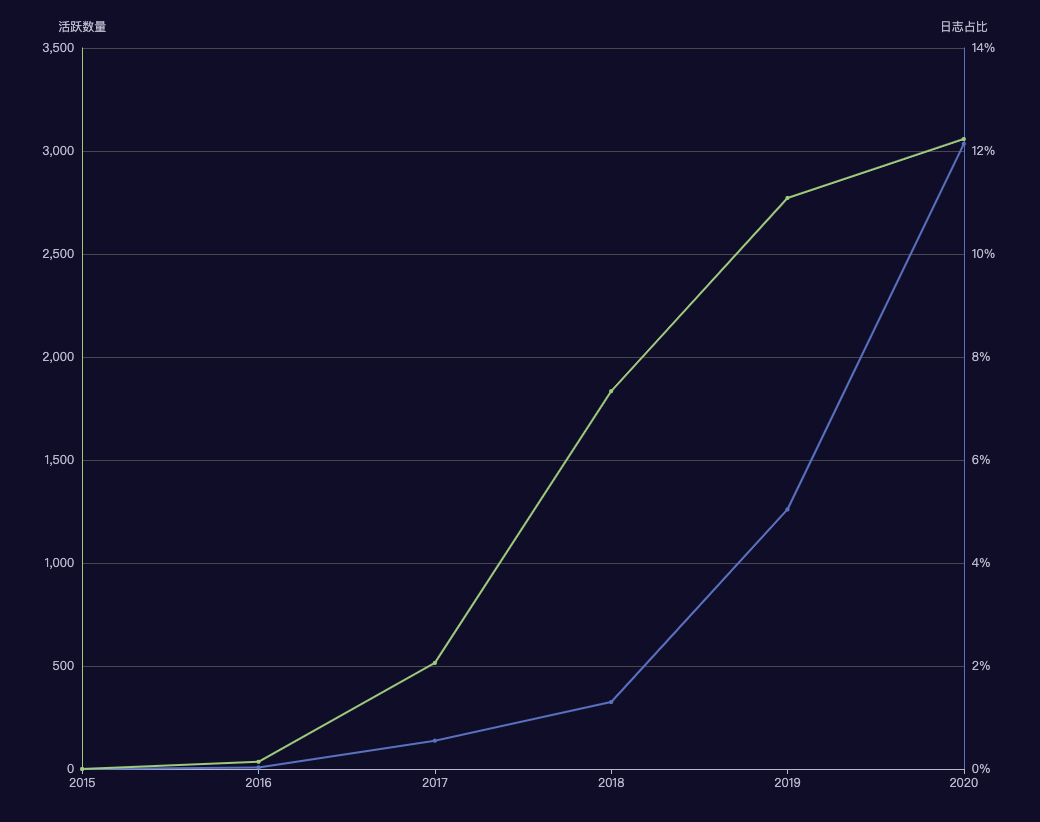
\includegraphics[width=130mm]{./figures/image1-2.png}
    \caption{GitHub Apps活跃账号数量与日志占比\\The number of GitHub Apps active accounts and the proportion of logs}
\end{figure}

\par 在这样的大环境之下,由华东师范大学与同济大学跨校组建的实验室X-lab设计并发起了一个面向开源项目的RPA(Robotic Process Automation机器人流程自动化)平台——Hypertrons,致力于向开源代码平台提供流程自动化定制与运行的能力。在开源社区中,Hypertrons扮演着开源项目和开放组织中的一个智能的数字劳工的角色,承担一些流程的自动的构建与编排,为跨平台的组织管理工作提供便利。在功能上,它依托于对全域开源行为的开放数据分析结果,帮助开发者与社区管理者进行决策,其方式是提供一个高度可配、高度可移植的框架,供用户在项目级别自定义组件,以配合不同项目的管理流程与制度。在开发者通常使用的各个平台(如Git、Gitlab、Github、Gitee、Slack、Jenkins、邮件、石墨文档和各类线上服务)之间,Hypertrons提供了跨平台交互的能力,同时为了更好地做出决策,也采集各平台的开放数据作为决策基础,为社区的数字化运营分析提供了有效的支撑。

\par 在Hypertrons项目中,不论是在项目层面对于用户行为数据的采集,还是将数据分析结果呈现给用户,都是一个无法避免地与用户产生联结、进行交互的过程。于是,为了更好地以交互的方式展现Hypertrons社区的数字化运营分析结果、辅助用户决策,面向开放组织的迷你看板项目应运而生。由于不希望深度改变用户的使用习惯,故发起一个浏览器插件项目,通过在特定网址的网页中插入迷你看板的方式为开放组织提供有效的监控和运营手段,这个项目是Hypertrons一大创新,也是Hypertrons的前端展示模块与功能延伸,即重要的组成部分。


\subsection{拟解决的主要问题}
% 思路:
% Hypertrons 没能做到的事情(或hypertrons与本项目的关系)

\par 一方面,迷你项目看板作为Hypertrons在浏览器端的入口之一,是Hypertrons的多平台集成与扩展能力的展示与增强。另一方面,通过该项目,可以非常方便且低成本地进行精细化市场运营:掌握用户的行为数据和兴趣偏好等重要信息,从而针对不同用户进行个性化的数字运营。

\par 经调研,在目前的各大代码托管平台中,仅项目页面会显示一些低阶指标数据(如Star数、贡献者列表等)与有限的的高阶指标数据(如GitHub Insights页面)。使用这些平台自带的功能,用户无从了解更多的高阶数据指标(如项目活跃度、流行度、贡献者活跃度、Issue平均响应时间等),从而无法很好或快速地掌握项目状况,进行管理或协同工作。而市面上已有的同类型看板应用,虽然也有用于项目健康度衡量分析的指标,但它们都以独立部署的平台、网站的形式呈现,无法很好地在此场景下为不同角色、不同平台的用户服务。于是,以浏览器插件形式存在的迷你看板成为了该场景下的一种更优解。

\par 根据Hypertrons的需求与迷你项目看板的产生动机,本课题关注的主要问题有两个:一是如何将开源社区中的开放数据进行分析呈现,即,可视化给用户;二是提供一种简单易用的交互方法,接收用户管理与配置的定制化指令(也即用户行为数据)。

\subsection{论文组织}

\par 本文在第一章介绍了课题的相关背景与产生动机,对应地提出拟解决的主要问题;在第二章中,将展开讲述如何对开源社区中的开放数据进行分析,包括了从数据的获取、探索性分析到数据预处理的流程;接下来的第三章,会根据前面分析得到的指向性信息,对不同业务场景实施数据设计;而第四章则从技术的角度,详述了面向开放组织的迷你看板应用的整体实现细节。     %正文第一章
\section{开源社区中的开放数据分析}

\subsection{数据的获取}
% GH Archive项目;
% Github事件日志、20种事件类型;
% ​更新周期:1周
\par 在世界范围内,开源开发人员同时在贡献着数百万个项目,为项目编写代码和文档、修复Bug、提交,而GH Archive 就是其中一个起到了记录作用的项目。它会记录公共的 GitHub 时间线,即按时间顺序录入GitHub 上所有行为活动的日志、存档,并使其能够被访问。本课题就使用了来自GH Archive的数据,开展进一步的研究。

\par 开源平台GitHub提供了 20 多种事件类型,范围从新的 Commit 和 Fork 事件,到提交新的 Pull Request、Comment 以及向项目添加成员。这些事件被聚合到每小时的存档中,自动更新,能够通过 HTTP 的方式访问获取。

\par 在本课题中,为了有效地进行开源项目或个人开发者的健康度衡量分析、呈现,在更新代价与数据有效性之间进行了折中选择,以1周为周期更新数据。

\subsection{数据预处理}
% 界定范围:Github全域;(还是仅活跃部分?)
% ​去除bot的极端数据
\par 为了能够更全面的了解开源社区的数据特征,同时保证其对当下情况较好的描述作用,在此选择了开源平台Github的2020年度全域数据作为样本,进行预处理以待进一步探索分析。

\par 在所有的数据中,由于Github Apps自动化协作机器人运行在服务端,可以同时服务于众多项目,从而具有了极高的活跃度和协作仓库数量,在后续统计开发者活跃度和活跃仓库数量时,对相关账号的协作行为进行了过滤。识别方法也很简单,即根据用户名后缀的[bot]进行账号识别。



\subsection{开放数据分析}
% 1. 全域开发者活跃情况:总体增长
% ​2. 开发者具有时区性:
% 3. 开发者使用语言分布:个人发展路径
% ​4. 项目中、项目间协作存在关系:开源进度不一,孤岛的存在,OpenGalaxy的评价标准(要放在这个部分吗?)
\par 从总体数据来看,2020 年全年的GitHub 全域事件日志数量总计约 8.6 亿条,较 2019 年 6.1 亿条增长约 42.6\%,是近五年来增长最快的一年。
% 既然目标是全域数据,这里使用Github2020的数据集进行分析是否合适?
经统计,2020年GitHub 全域活跃项目数量约 5,421 万个,活跃开发者账号约 1,454 万,分别较 2019 年增长 36.4\% 与 21.8\%。通过对全域开发者进行活跃度与活跃仓库数量的统计,可以得到 GitHub 全域开发者的活跃度分布情况和单个开发者活跃仓库数量分布情况如下:
\begin{figure}[H]
    \centering
    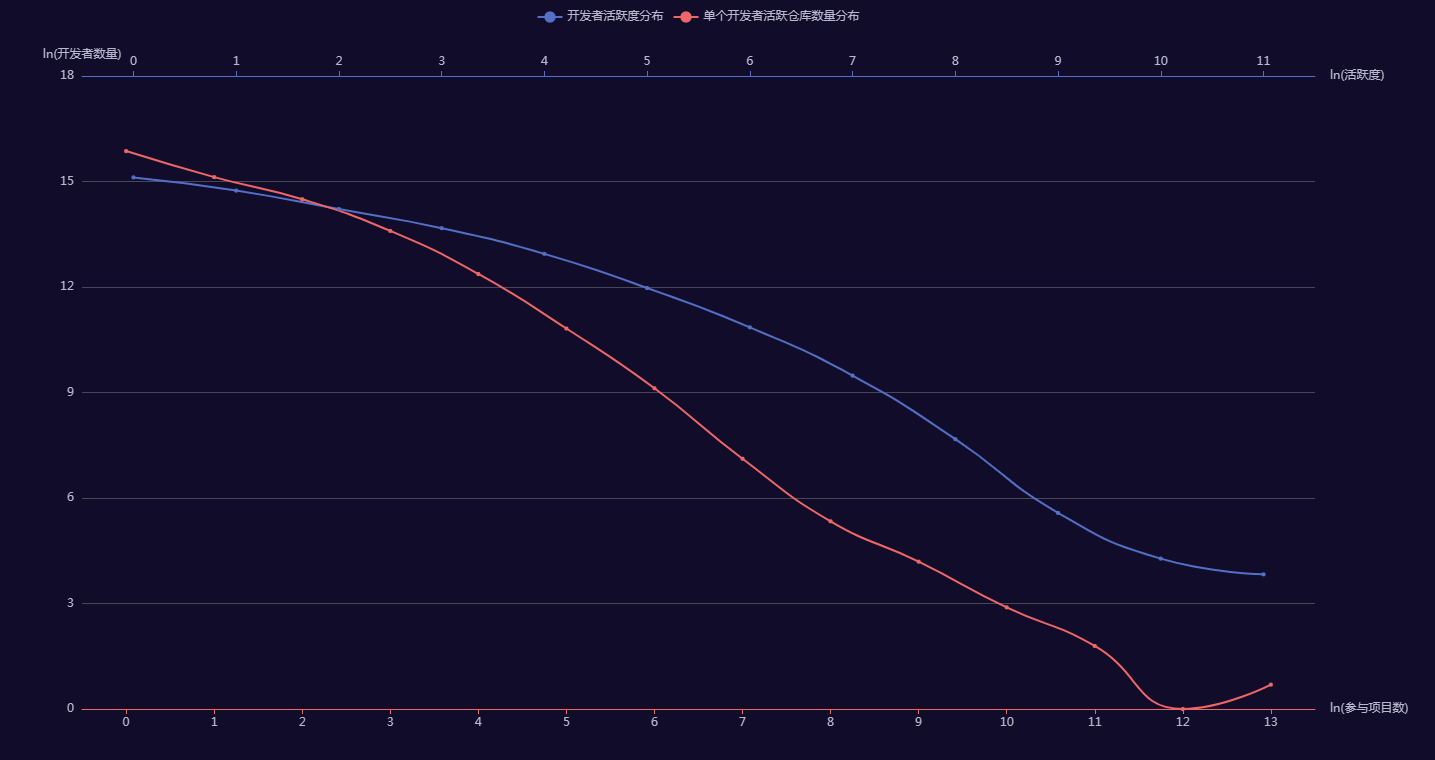
\includegraphics[width=130mm]{./figures/image2-1.png}
    \caption{开发者活跃度与活跃仓库数量分布图\\Figure 3-1: Distribution diagram of developer activity and the number of active warehouses}
\end{figure}

\par 图2-1使用双对数坐标系绘制,图上方的横坐标表示开发者活跃度,图下方横坐标表示开发者参与项目数量,纵坐标表示开发者数量,所谓双对数坐标,就是将原来的线性坐标轴都取自然对数,可以看到开发者活跃度与活跃仓库数量的分布符合幂律分布。经统计,活跃度超过 2,000 的开发者数量为 5,445 个,占全域开发者数量不足万分之六。而大部分开发者活跃度都在 [0, 500] 区间内,占全域开发者数量的 99.45\%,说明大多数开发者还是处于低活跃度的一个状态。观察曲线尾部,我们发现开发者活跃仓库数量在最后有一个回升,其实是由于部分未被过滤掉的自动化协作类账号的活跃仓库数量巨大,远超正常人类开发者,因此尾部形成V形曲线。

\par 由于开源开发者在地理位置上遍布全球,他们具有不同的工作时间分布情况。通过对Github事件日志的详细时间戳数据可视化,可以看到在UTC标准时间下,全球的开源开发者工作时间分布具有明显的规律,如图2-2所示,横轴为一天 24 个小时(UTC标准时间),纵轴为一周 7 天,圆点大小表示该时段项目内产生的日志量的总和。
\begin{figure}[H]
    \centering
    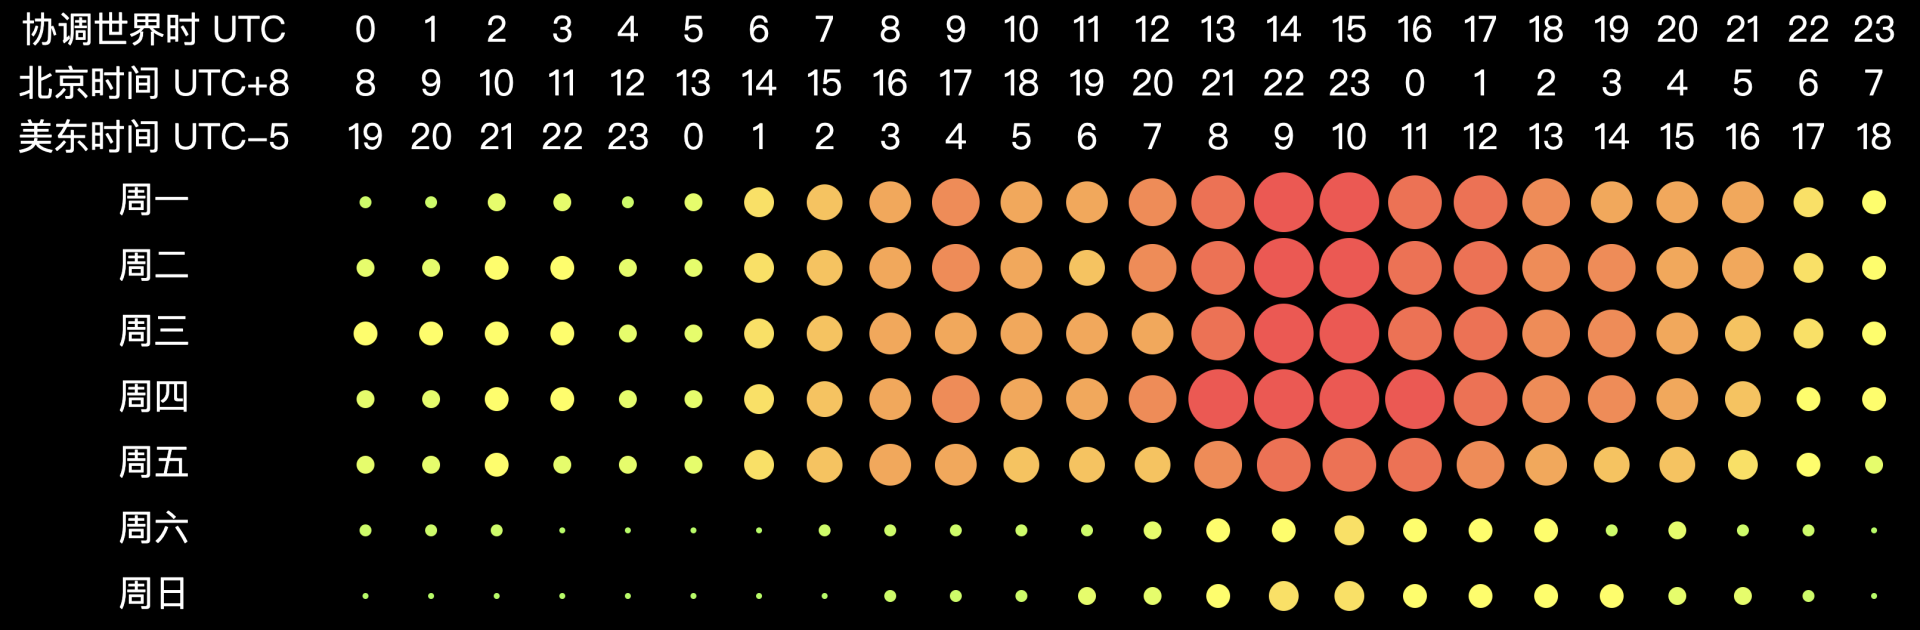
\includegraphics[width=130mm]{./figures/image2-2.png}
    \caption{GitHub 2020 年全球日志时间分布情况\\Figure 3-2: The global log time distribution of Github in 2020}
\end{figure}

\par 如果从日志中抽取每个开发者独立的日志在每日不同时间段的分布情况,并通过对开发者进行时区估计后将其移动合并到同一时区,就能够得到开源开发者的典型工作时间分布情况,从而推断出开发者所属时区、地区,或是根据项目成员的协作时间分布,来判断一个项目的国际化程度。如图2-3所示,对项目内部所有开发者进行时区估计,随后以UTC标准时间下的24个时区为横轴,以每个时区开发者比例为纵轴,作分布直方图。
\begin{figure}[H]
    \centering
    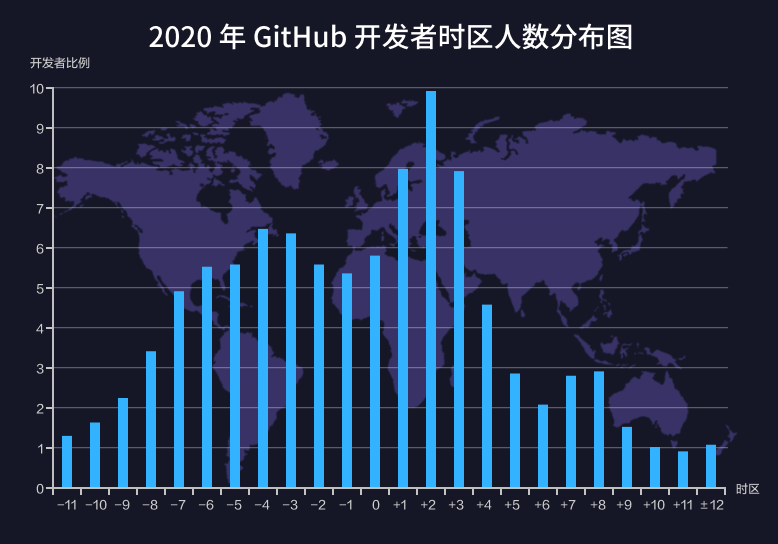
\includegraphics[width=90mm]{./figures/时区分布.png}
    \caption{GitHub 2020 年全球开发者时区人数分布图\\Figure 3-3: GitHub global developer time zone distribution map in 2020}
\end{figure}

\par 开发者的地理分布情况一直是开源项目全球化指标的一个重要方面,然而一直以来没有较好的方式来估计开发者所在时区,但在全域日志数据下,开发者的个人行为为我们提供了有效的估计手段。可以在全域范围或特定开发者群体内估计开发者在不同时区的占比情况,从而有效判断 GitHub 全域或特定项目内的全球化覆盖情况。

\par 另一方面,在不同的项目中,开源开发者们会使用不同的语言,也具有着一定的技术学习路线\cite{dabbish2012social},即主要使用的语言事件数量产生明显的增、减变化。在开源社区,由个体语言选择产生的变化组成了社区开发语言迭代的趋势,反之,开发语言的流行趋势也影响着开发者的学习路径。根据开源社区中活动频繁、贡献最大的一批用户的学习路径,就可以形成全域开发语言的流行趋势预测,从而为开发者的发展提供参考。
\begin{table}[htbp]\center
    \caption{GitHub 2020 年全域活跃开发者和 Top10 万活跃开发者语言分布对比\\ Table 3-1:  Comparison of the language distribution of GitHub's global active developers and the top 100,000 active developers in 2020}
    \begin{tabular}{|c|cc|cc|}
        \hline
        排名 & 全域开发者语言榜 & \makecell*[c]{全域范围\\开发者账号数} & \makecell*[c]{Top 10万开发者语言榜} &\makecell*[c]{Top 10万范围\\开发者账号数}\\
        \hline
        1 & JavaScript & 305,814 & JavaScript & 15,858 \\
        2 & Python & 175,610 & Python & 10,866 \\
        3 & HTML & 159,303 & TypeScript & 7,419 \\
        4 & Java & 139,673 & Java & 6,665 \\
        5 & Ruby & 87,780 & Go & 5,094 \\
        6 & TypeScript & 85,116 & C++ & 4,204 \\
        7 & C\# & 54,343 & Ruby & 3,802 \\
        8 & PHP & 52,915 & HTML & 3,490 \\
        9 & C++ & 47,799 & PHP & 3,000 \\
        10 & CSS & 46,428 & C\# & 2,892 \\
        \hline
    \end{tabular}
\end{table}
\par 将2020年全域所有活跃开发者使用的语言分布和活跃度 Top 10 万的开发者使用的语言分布情况进行对比,可以看到存在着一定的区别,如表3-1所示。

\begin{figure}[H]
    \centering
    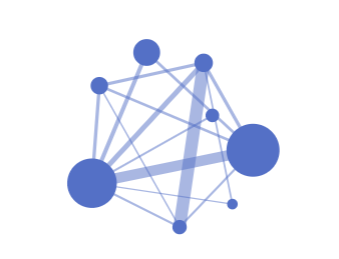
\includegraphics[width=80mm]{./figures/开发者协作网络图.png}
    \caption{某项目的开发者协作网络图\\Figure 3-4: The developer collaboration network diagram on a repository}
\end{figure}

\par 除了个体之间的差异,不同的开发者之间也存在着协作关系\cite{廖志芳2019github开源软件开发过程中关键用户行为分析}。在某一开源项目中,来自不同开发者的贡献使他们构成协作网络,如图3-4所示,对于在该项目中作出贡献的开发者,取top N位(N由用户定义配置)生成网络图,图中节点描述各开发者,节点大小描述开发者对该项目的贡献量,节点之间边的粗细描述两个开发者之间的协作活跃度\cite{thung2013network}。

\par 同一位开发者又有可能参与了多个项目,于是项目与项目之间也具有了关联性。综上两个方面考虑,优秀的开发者对项目具有着影响力,同时优秀项目更容易聚集优秀的开发者,这两者之间相互具有作用力。这样的关系可以用协作网络来进行可视化描述,通过项目协作关联度和社区发现算法对项目进行聚类,从而得到基于协作行为的聚类效果,并用于项目的大致分类。

\par 根据连通性分析,在全域约 105 万个开源项目中,共分成了 44,990 个连通子图,其中 935,231 个项目在协作关系下构成一个巨大连通子图,其他 44,989 个连通子图中最大的子图包含 200 个项目,最小的包含 1 个项目,包含了 100 个项目以上的连通子图仅 9 个。这意味着全域活跃项目中 89\% 的项目构成了一个巨大的协作网络,也就是 GitHub 开源世界的核心。而另外还有将近 4.5 万个小的协作孤岛,这些小的协作网络与开源世界不连通,意味着这些项目上的所有开发者都仅在自己的项目群中协作,从未在其他项目上有过活跃行为,同时在开源核心中的任意开发者也都没有在这个项目群中产生过协作行为\cite{刘玉辉2018github}。


        %正文第二章
\section{面向开放组织的数据信息挖掘框架}
% 从Github全域数据中能提取到什么信息,即看板展现的内容。【数据结构】(这里要直接讲数据结构吗?】
% 意义:
% 快速挖掘出项目中的深层信息
% 帮助开源项目的管理
% 帮助个人职业规划与发展
% \par 上一章中,对开源社区中开放数据的探索性分析从社区活跃情况、开源开发者的工作时间分布、开发语言的使用、项目或开发者之间的协同关系四个角度,带来了对项目或个人开发者行为的更深层解读,揭露了开源社区庞大的开放数据中所含信息量的冰山一角。如果这些信息能够被快速挖掘、定向展现,那么将大大助益开源社区的发展。

\par 对于开源开发者而言,通过个人行为数据的汇总挖掘,能够更好地自我了解与进行职业规划;对于开源项目而言,这些数据将提供不同的维度来评估其影响力、国际化程度,即便对于项目不熟悉的人,也能在很短的时间内快速了解项目状况,更可以方便项目管理与社区治理\cite{kalliamvakou2014promises}。


% \subsection{衡量指标定义}
% 活跃仓库与开发者统计方法;
% ​开发者活跃度;
% ​项目活跃度;
% 时区估计方法;
% 主要开发语言;
% ​开发者协作网络构建方法;
\subsection{活跃仓库与开发者统计方法}
\par 若被统计的代码仓库包含事件日志,仓库即被定义为活跃仓库;若开发者有任意代码仓库包含事件日志,开发者即被定义为活跃开发者。

\subsection{开发者活跃度}
\par 开发者活跃度,其定义为某特定 GitHub 账号在一段时间内在某特定 GitHub 项目中的活跃评价指标。其活跃度由该账号在该项目中的行为数据决定,本文中所关心的行为包含如下几种:\cite{王伟2020全球开源生态发展现状研究}

\begin{itemize}
    \item Issue comment:在 issue 中参与讨论是最基本的行为,每个评论计入 1 次。
    \item Open issue:在项目中发起一个 issue,无论是讨论、bug 报告或提问,对项目都是带来活跃的,每个发起的 issue 计入 1 次。
    \item Open pull request:为项目提交一个 PR,表示已对该项目进行源码贡献,则每次发起一个 PR 计入 1 次。
    \item Pull request review comment:对项目中的 PR 进行 review 和讨论,需要对项目有相当的了解,并且对项目源码的质量有极大帮助,每个评论计入 1 次\\
          注:仅通过代码 review 对特定代码行的讨论记为 review,直接对 PR 的评论回复记为 issue comment 事件。
    \item Pull request merged:若有 PR 被项目合入,即便是很小的改动,也需要对项目有较为深入的理解,是帮助项目进步的真切贡献,则每有一个 PR 被合入计入 1 次,同时 PR 合入事件根据该 PR 的代码增加行数。
    \item Watch:用户 star 项目,被计入 1 次。注:Star 操作在 GitHub 日志事件中记为 Watch 事件。
    \item Fork:开发者 fork 该项目,被计入 1 次。
\end{itemize}

以上 7 个种行为各自独立计数,具有不一样的权重,根据专家经验,加权值分别为 1、2、3、4、2,1,2,即:
$$
 A_{u\_d}=C_{issue\_comment}+2{C}_{open\_issue}+3{C}_{open\_pr}+4{C}_{review\_comment}+2{C}_{pr\_merged}+{C}_{watch}+2{C}_{fork} 
$$
其中,Pull request merged 的计数由分段函数决定\cite{tsay2014influence}:

$$ C_{pr\_merged}=\left\{
    \begin{array}{rcl}
        0.8+0.002 \times loc &  & {loc < 100}          \\
        1                    &  & {100 \leq loc < 300} \\
        2.5-0.005 \times loc &  & {300 \leq loc < 400} \\
        0.5                  &  & {loc \geq 400}
    \end{array} \right.
$$

其中,loc 表示新增的代码行数。根据软件计量学经典数据统计,单次代码变更最佳在 200 行以内,超过 400 行的代码变更会导致审阅困难,故通过分段函数关联了代码新增行数与 PR 的权重指标。

\subsection{项目活跃度}
\par 项目活跃度定义为某特定项目在一段时间内的活跃评价指标。其活跃度由单开发者在一天内的活跃度加总计算得到(时间点与时间段计算方式均基于开发者个人活跃度方式计算):

$$ A_{r} = \sum (A_{u\_d} / day\_count) $$

开发者活跃仓库数量,则在此基础上定义为,由每个开发者所产生的活跃度大于 0 的仓库数量。

\subsection{开发者时区估计方法}

\par 根据开发者全年每小时产生日志的数量,计算获取其事件最多的连续 12 个小时,令其时间为该开发者本地时间的 9 时至 21 时,则可以大致确定该开发者的所属时区。因为日志所记录的时间为 UTC 标准时间\footnote{
UTC 即协调世界时间,是国际通用的时间标准,将全球各地的时间进行同步协调。UTC 时间是经过平均太阳时(以格林威治时间 GMT 为准)、地轴运动修正后的新时标以及以秒为单位的国际原子时进行综合精算而得到的。
世界时区使用 UTC 的正或负偏移量表示。最西端的时区使用 UTC-12,比UTC落后十二小时;最东部的时区使用 UTC+14,比 UTC 早 14 小时。出现 UTC+13,UTC+14 的原因如下:
    \begin{enumerate}
        \item[1)] 因为国际日期变更线,虽然1884年划定时避免在一个国家中同时存在着两种日期,但是1979年成立的基里巴斯领土却跨越了国际日期变更线。基里巴斯的UTC有:莱恩群岛(UTC+14)、菲尼克斯群岛(UTC+13)、吉尔伯特群岛(UTC+12),这样保证一个国家内的日期为同一天。
        \item[2)] 因为夏令时,即天亮早的夏季人为将时间调快一小时。比如新西兰是 UTC+12,在夏时制改用 UTC+13。
    \end{enumerate}
北京时间是中国采用国际时区东八时区的区时作为标准时间,东八区(UTC+8)是比 UTC 早 8 小时的时区。
}。考虑开发者一天连续 12 个小时产生日志数最多的最后一个小时,其最后一小时(即本地时间 21 时)对应的 UTC 时间记为 $ k $, 则时区计算公式如下:
$$
    zone=
    \begin{cases}
        20-k^*, & k^*>8 \quad \text{对应本地为东时区}     \\
        -4-k^*, & k^*\le 8  \quad \text{对应本地为西时区}
    \end{cases}
$$

\par 其中,数学公式: $ k^*=argmax\{\sum_{i=k-11}^{k}{c_i} \},\quad  k=0,1,...,23 $, $ c_i $表示当前小时产生的日志数量。当 i 为负值时,意味着为前一天的时间,需进行转换,即使用数学公式: $ i=i+24 $进行转换。

\par 因单个开发者的行为具有偶发性与特殊性,本方法不可用于单开发者时区的精确估计,但其在统计维度上具有意义,在此仅考虑统计学意义。再者,活跃度较低的开发者,其行为发生也具有偶发特性,所以在对开发者时区判断时,剔除了 GitHub Apps 并只保留全域活跃度排名前 5 万名的开发者账号用于分析,得到的工作时间画像如图2-3所示。

\begin{figure}[H]
    \centering
    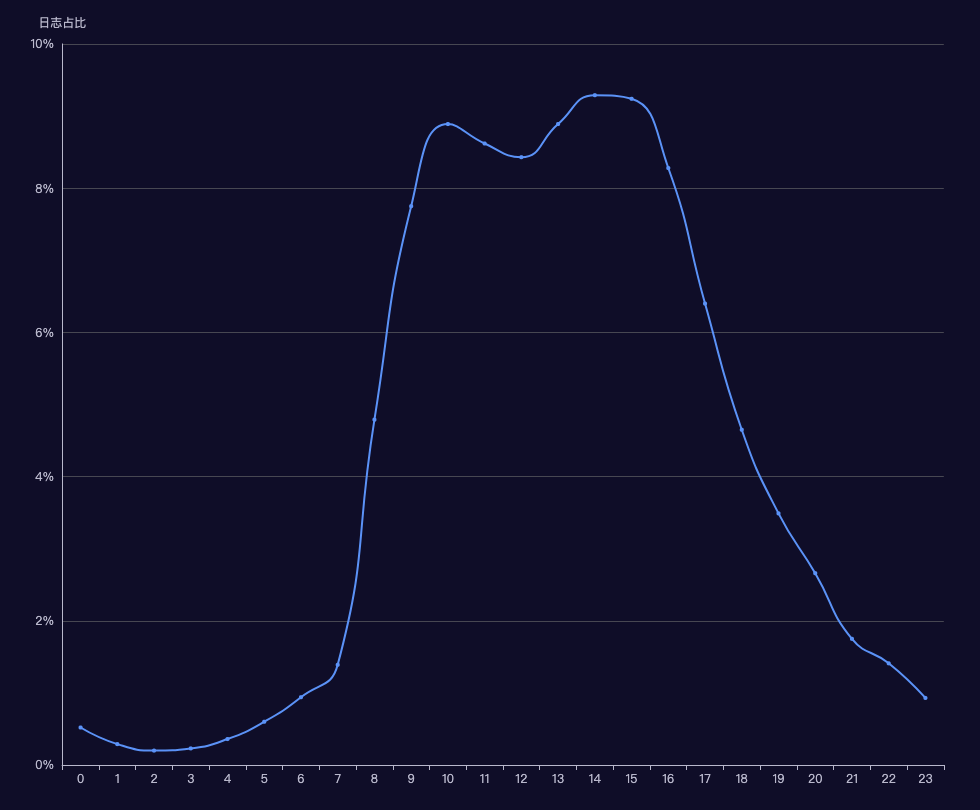
\includegraphics[width=130mm]{./figures/image2-3.png}
    \caption{ 典型开源开发者工作时间画像\\Figure 2-1: Portrait of a typical open source developer's working hours}
\end{figure}

\par 由图2-3所示,开发者通常会选择从当地时间早上 8 时开始工作,中午 11 - 13 时进行短暂的午休,随后在下午 15 - 16 时达到一个生产力高峰,并持续产出到晚间,较符合常见的工作时间情况;另一方面,可以看到开发者在晚间的工作产出比例还是较高的,甚至可以工作到凌晨 1 点,活跃程度应该明显高于一般职业。

\par 在高活跃开发者中,UTC-8 至 UTC-3,即美洲(美国、加拿大、南美)开发者分布最多,虽然单时区的开发者比例不是最高,但总体开发者占比高达 33\% 左右。而 UTC+1 至 UTC+3,即欧洲拥有最高的单时区开发者比例,UTC+1 时区高达近 10\%,三个时区的总占比约为 26\% 左右。总体而言,亚洲的开发者数量依然较少,但在 UTC+7 至 UTC+8 区域有一个小的波峰,说明中国、俄罗斯开发者相较其他国家还是有较高的开源活跃。而太平洋地区(UTC+9 至 UTC-9)则由于人口分布原因,开发者比例最低。


\subsection{开发者使用语言统计方法}
\par 开发者使用语言定义为一个开发者账号在该年度使用频率最高的语言,其具体实现为一个开发者账号在该年度提交并合入 PR 最多的项目所使用的主要编程语言。


\subsection{​开发者协作网络构建方法}
开发者协作网络是基于说明 2.1 中开发者活跃度的定义,通过多个开发者在项目中的协作关系进行构建的。具体构建过程为将每个开发者的全年活跃度计算精细化到具体的 issue/PR 之上,则同时在同一个 issue/PR 上有过活跃的开发者认为其具有协作关系,而协作关系与两人在该 issue/PR 上的活跃度相关,具体计算方式为:

$$ R_{ab}=\sum_{i}{\frac{A_{ia}A_{ib}}{A_{ia}+A_{ib}}} $$

其中 $ A_{ia}, A_{ib} $分别为开发者 a 和 b 在 issue/PR i 上的活跃度,计算方法遵循 2.1 中的开发者活跃度计算方法, $ R_{ab} $为开发者 a 和 b 在该项目上的协作关联度。即两个开发者在项目的协作关联度为其在所有共同活跃的 issue/PR 上的活跃度的调和平均值之和。
\subsection{开源象限分析}
\par 提出一种开源象限(OpenQuadrant)的方法来刻画一个开源项目在影响力、全球化、社区规模三个核心特性方面的表现。基于该开源象限分析,使用散点图来表示,横纵两个维度为项目影响力指标和项目全球化指标,为了方便可视化,我们采用取对数的形式呈现上述两个指标,而使用散点图上的点的大小来刻画项目参与的活跃人数,用来反映一个项目的社区规模。\cite{vasilescu2015quality}

\par 以2020年CNCF基金会( Cloud Native Computing Foundation,即“云原生计算基金会”)下云原生领域的开源象限分析结果为例,如图2-2所示,
\begin{figure}[H]
    \centering
    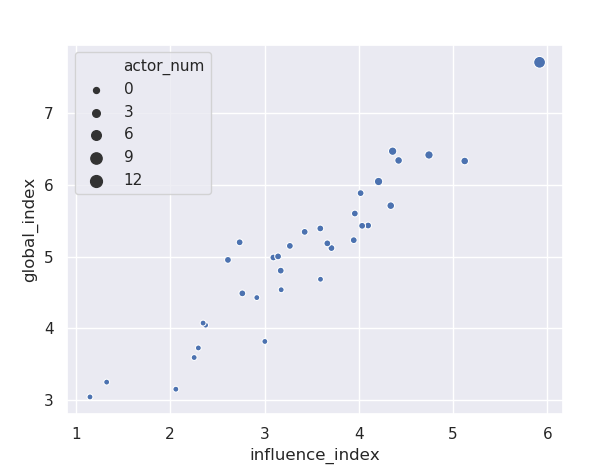
\includegraphics[width=100mm]{./figures/开源象限.png}
    \caption{CNCF 下云原生领域的开源象限\\Figure 2-2: Open source quadrant in the cloud native field under CNCF}
\end{figure}
基于以上,开源象限将整个平面分成了四块区域,分别是:
\begin{itemize}
    \item 前瞻(Foresighted):落在该区域的项目影响力强,同时项目全球化程度高;
    \item 引领(Leading):落在该区域的项目影响力强,但项目全球化程度较低;
    \item 行动(Acting):落在该区域的项目影响力较弱,但项目全球化程度高;
    \item 进入(Incubating):落在该区域的项目影响力较弱、同时项目全球化程度也较低。
\end{itemize}
\par 影响力、全球化、参与人数的具体计算方式如下所示。

\subsubsection{领域项目影响力指标}
% //TODO:领域项目影响力指标的定义
\par 领域项目的影响力计算结果是由全域项目的影响力计算结果给出,%计算方法参见上文 3.6 说明 1。

\subsubsection{领域项目全球化指标}
\par 全球化的影响因素众多,考虑地域、开发者人数这两个因素用于项目全球化指标的计算。针对地域因素,考虑计算参与该项目的开发者的时区分布情况,开发者时区分布趋于均匀分布,即标准差越小时,认为该项目的全球化程度越高。因此,首先通过判断项目上所有开发者的时区,之后计算了项目在 24 个时区上对应的开发者人数,在此基础上,计算项目关于时区人数的标准差。针对开发者人数因素,即该项目上参与的开发者总数,开发者人数越多,该项目全球化程度越高。考虑到开发者人数不多,但开发者的行为具有偶发特性的情况,该情况导致地域因素计算不准确,从而导致全球化指标的结果不准确。因此,使用如下全球化指标计算公式:

$$ \sqrt{\frac{24}{\sum_{i=-12}^{11}{(x_i-\bar{x})^2}}}\bar{x}^2, \quad x_i\text{表示该项目在i时区的开发者人数。} $$

\par 上述计算公式表明,全球化指标与项目时区开发者人数均值的平方成正比,与项目时区开发者人数的标准差成反比。该计算方式能够有效评估开发者人数较少的项目的全球化程度,另一方面,该计算方式对开发者人数较多的项目,全球化指标计算有正向作用。

\subsection{项目参与人数}
\par 项目参与人数,即在项目上发生日志行为的参与者总数。在可视化散点图点的处理上,我们对领域项目的参与人数使用线性最大最小归一化,使得数值映射到了1-10区间范围内\cite{mcdonald2013performance}。


% \subsection{数据设计}
% \subsection{开发者分析方法}
% \par 以某开发者数据为例,取半年作为时间区间,设计如下图表:

% \subsubsection{个人活动}
% % 开发者活跃度-折线图
% % 工作时间分布-打孔图
% % Github事件雷达图
% \paragraph{开发者活跃度} 以时间为横坐标,以开发者活跃度为纵坐标,展示形式为折线图。

% \paragraph{工作时间分布} 横轴为一天 24 个小时(UTC标准时间),纵轴为一周 7 天,圆点大小表示该时段产生的日志量的相对大小。

% \paragraph{事件雷达图} 以该开发者的Star、Fork、Commit、OpenIssue、OpenPR、PR review事件次数作雷达图。

% \subsubsection{个人发展}
% % 语言使用分布-百分比堆积条形图
% % 个人关注点-Issue label词云
% \paragraph{语言使用分布} 将用户的各项目仓库中占比最大的语言作为该项目的开发语言,统计用户所有项目语言种类,并计算占比,以百分比堆积条形图的形式呈现。

% \paragraph{个人关注点} 在开放平台的issue板块,用issue做任务划分和bug记录时,项目管理人员或issue的发起者常常使用标签来给issue做标注,以便于区分issue类型,这种标签便被称为issue label。统计个人开发者参与或发起的issue所带issue label,按出现频率生成词云,能够展现该开发者在开发过程中的个人关注点。

% \subsubsection{协作关系}
% % 开发者协作-网络图
% % 项目关联-网络图
% \paragraph{开发者协作网络} 凡是与某开发者之间协作活跃度$R_{ab} > 0$ 的开发者,取top N位(N由用户定义配置)生成网络图,图中节点描述各开发者,节点大小描述开发者活跃度,节点之间边的粗细描述协作活跃度。支持交互式访问,点击节点跳转至协作者的主页。

% \paragraph{关联项目网络} 在开发者作出commit、PR贡献的所有项目中,取top N个项目(N由用户定义配置)生成网络图,图中节点描述各项目,节点大小描述用户对该项目的贡献量。
% % TODO: 贡献怎么定义的?节点间有无连接?
% % 贡献量:开发者对项目所作出的活跃度的贡献,开发者在这个项目的活跃度/项目活跃度

% \subsection{项目分析方法}
% \par 以某项目数据为例,取半年作为时间区间,设计如下图表:
% \subsubsection{项目生命力}
% % 活跃度-曲线图
% % 一周commits、star、fork-复合曲线
% % 参与度
% %   打开/关闭的issue-双向柱状图
% %   代码行数变化-双向曲线图
% % 项目回应度基于每日issue和pr的初次响应时间
% %   PR平均解决周期(每月)-热力图
% %   Issue平均响应时间-?
% \paragraph{项目活跃度} 以时间为横坐标,以项目活跃度为纵坐标,展示形式为折线图。在此基础上复合以每周commit、star、fork数量为纵坐标的堆叠折线图。
% \paragraph{issue状态} 以周数为横轴,以每周的issue数量为纵轴,向纵轴的正、负方向分别作打开、关闭状态issue的双向柱状图。
% \paragraph{代码行数变化} 以时间为横轴,以每天的代码量增减行数作为纵轴,向纵轴的正、负方向分别作代码增加、减少行数的双向曲线图。
% \paragraph{PR平均解决周期} 
% % TODO: 纵轴是什么
% \paragraph{Issue平均响应时间} 


% \subsubsection{项目多元化}
% % 参与人数与New Contributer的数量-百分比堆积条形图
% % 工作时间分布-打孔图
% % 开发者时区分布-柱状图
% \paragraph{参与人数与New Contributer的数量} 定义最近一周内参与贡献的开发者为该项目的New Contributer,统计项目所有的参与人数与New Contributer数量,并计算占比,以百分比堆积条形图的形式呈现。
% \paragraph{工作时间分布} 根据事件日志的时间戳作打孔图,横轴为一天 24 个小时(UTC标准时间),纵轴为一周 7 天,圆点大小表示该时段项目内产生的日志量的总和。
% \paragraph{开发者时区分布图} 对项目内部所有开发者进行时区估计,随后以UTC标准时间下的24个时区为横轴,以每个时区开发者比例为纵轴,作分布直方图。

% \subsubsection{协作的力量}
% % 开发者协作-网络图
% % 关联项目-网络图
% % 一周活跃开发者榜单(top N)-List
% % 开发者留存率-?
% \paragraph{开发者协作网络} 对于在该项目中作出贡献的开发者,取top N位(N由用户定义配置)生成网络图,图中节点描述各开发者,节点大小描述开发者对该项目的贡献量,节点之间边的粗细描述两个开发者之间的协作活跃度。支持交互式访问,点击节点跳转至协作者的主页。

% \paragraph{关联项目网络} 对于参与该项目的开发者作出commit、PR贡献的其他项目,生成网络图,图中节点描述各项目,节点大小描述项目活跃度,节点之间边的粗细描述项目之间的相关性。
% % TODO: 项目间的相关性是怎么定义的?
% \paragraph{一周活跃开发者榜单} 在本周活跃开发者中取top N(N由用户定义配置)个,按贡献度顺序形成列表。列表包含开发者id与贡献度。


% \subsection{社区分析方法}
% \par 上文中对于项目的分析方法也同样适用于社区分析,唯一的不同在于社区分析的数据来源于社区组织下所有项目的事件日志总和。在此基础上,再对社区分析增加以下方法。
% \subsubsection{开源象限分析}
% % 影响力、全球化、社区规模
% 提出一种开源象限(OpenQuadrant)的方法来刻画一个开源项目在影响力、全球化、社区规模三个核心特性方面的表现。基于该开源象限分析,使用散点图来表示,横纵两个维度为项目影响力指标和项目全球化指标,为了方便可视化,我们采用取对数的形式呈现上述两个指标,而使用散点图上的点的大小来刻画项目参与的活跃人数,用来反映一个项目的社区规模。

% 基于以上,开源象限将整个平面分成了四块区域,分别是:
% \begin{itemize}
%     \item 前瞻(Foresighted):落在该区域的项目影响力强,同时项目全球化程度高;
%     \item 引领(Leading):落在该区域的项目影响力强,但项目全球化程度较低;
%     \item 行动(Acting):落在该区域的项目影响力较弱,但项目全球化程度高;
%     \item 进入(Incubating):落在该区域的项目影响力较弱、同时项目全球化程度也较低。
% \end{itemize}




      %正文第三章
\section{面向开放组织的迷你看板设计}
\subsection{需求设计}
\par 当前,由于代码托管平台仅在项目或个人主页上呈现低阶的指标数据和有限的高阶指标数据,用户无法查看自定义的高阶指标数据,从而无法在较短时间内深入了解该项目或用户。面向开放组织的迷你看板最主要的目的与动机是直观清晰地展示项目高阶指标数据,并让这种可视化展现与项目本身无缝结合,充分发挥其助力能力,让用户能够轻松地把握各项项目“体征”,降低心智成本。在这一方面,对市面上已有的同类型看板应用进行调查,发现它们大都以独立的平台、网站的形式呈现,用户跨平台操作具有一定的门槛,且这样呈现的效果的直观程度大打折扣。

\par 从另一个方面,作为Hypertrons的前端拓展,迷你看板可以改善Hypertrons的使用体验,补全Hypertrons在浏览器端的交互能力,为用户带来更加快速的开发、协作体验。比如,在Hypertrons项目中,存在一些场景下的交互指令(如self-assign 等命令)需要手输,容易致使用户忘记或输入错误,但如果看板应用将手输代码指令这一个动作包装成为一个前端页面的按钮点击动作,那么用户就可以更快更好地达成操作。%//TODO:另外,在权限管理方面,无法对具有高权限的用户也实施自行代码合并、 PR review 机制等良好的社区规范,即:有权限的用户仍然可以自行合并代码;

\subsection{总体设计}
% \subsubsection{产品定位}
% chrome extension:由于不希望深度改变用户的使用习惯,故发起一个浏览器插件项目,通过在特定网址的网页中插入迷你看板的方式为开放组织提供有效的监控和运营手段。
% 目标:
% ​直观清晰地展示项目高阶指标数据,与项目本身无缝结合,让用户轻松把握各项项目“体征”,降低心智成本。
% 改善 Hypertrons 使用体验,补全 Hypertrons 在 Browser 端能力,为用户带来更加便捷的开发、协作体验
\par 根据以上需求分析,面向开放组织的迷你看板其最主要的目的是辅助开源社区,并不希望深度改变用户的使用习惯,故在产品定位上,选择了浏览器插件的形式。该浏览器插件将运行在网页端,通过检测当前浏览页面url的方式,为带有特定域名(目标开源平台域名)的网页插入迷你看板,并提供可以由用户自定义的图表设置选项,达到向开放组织提供有效的监控和运营手段的最终目标。


\subsection{功能设计}
% 【用户角度、业务逻辑】
% 高可配的数字化看板
% 跨平台交互
% 实时消息通知
% 配置管理
% 身份认证与权限管理
\subsubsection{高可配的数字化看板}
\par 数字化看板即在前端页面插入的可视化图表部分,也是该插件的最主要功能。它面向不同身份的用户,根据用户设置来展示定制的图表内容。当浏览器加载开源平台的页面时,插件将根据所加载页面对应的数据分析方法(个人主页对应3.2、项目主页对应3.3、组织主页对应3.3),提供用于分析的几个维度所对应的所有图表;而用户则在插件设置选项中选择性地开启或关闭特定图表,以达到定制化的目的。
\par 特别地,在项目主页中,根据用户角色模型将用户分为User 、Contributor、Committer。在针对不同用户展示个性化的项目情况数字看板时:
a.	如果当前用户为User,则展示该项目的基本信息,如Star数、Contributor数、软件下载数等,帮助用户建立对整个项目的初步的整体认识。同时可通过一定的手段吸引并将该用户转化为贡献者,例如,列出标签为“good-first-issue”的Issue列表,引导用户为该项目做贡献。
b.	如果当前用户为项目的Contributor,则展示该名贡献者过去一段时间的贡献列表(Issue 或PR等),并显示该用户所贡献的Issue或PR的最新动态,同时鼓励用户持续贡献。
c.	如果当前用户为项目的Committer,则监控与项目健康度相关的一些指标,如 Issue 或 PR 的相应时间、项目贡献者及隶属组织多样性等,帮助 Committer 建立对项目现状及演化趋势的整体把握。
d.	如果当前用户为项目的运营人员,则可以展示与项目运营活动相关的指标。


\subsubsection{跨平台交互}
\par 跨平台交互在本项目中指:来自不同系统、平台的用户,都可以在前端页面中实时地输入特定的指令来获取相应的支持,而不需要配置对应的本地环境,如:在浏览器页面键入/help指令查看帮助,或使用受支持的/sendMsg指令向其他平台发送自定义消息。

\subsubsection{跨平台实时消息通知}
\par 通过浏览器的消息通知机制,可以提供跨平台消息实时通知能力。例如,当项目发布新版本或者有其他新闻通知时,hypertrons 后端将消息推送给所有已安装的拓展程序,浏览器的消息服务将会唤醒用户安装的拓展程序,由拓展程序分析得到的消息数据,并创建通知,这样,不同身份的用户即可收到个性化的消息通知。

\subsubsection{配置管理}
\par 用户可以在扩展程序的菜单栏中对配置进行修改,例如是否启用数字化看板、跨平台交互以及跨平台实时消息通知等功能。另外,可以考虑支持用户对本地页面的数字化看板进行配置,将这些配置存放于本地,覆盖默认的看板配置。

\subsubsection{身份认证与权限管理}
\par 身份认证与权限管理是 Hypertrons 的核心功能之一。迷你项目看板可在浏览器前端页面中为用户提供身份认证入口,引导用户前往相关平台进行 Oauth 认证,并将用户的身份认证信息保存至 Hypertrons 后端,为用户行为数据分析与精细化运营提供基础。同时,为了支持用户进行跨平台交互操作,可支持用户在扩展程序中配置不同平台的 Token。


\subsection{运营方式}
% 三个会员等级付费制度,Basic做引流,Detailed展示项目/开发者细节和基础数据聚合,Advanced展示高级指标和深度分析结果
\par 迷你看板插件的安装与使用是开源并免费的,但对看板的可视化内容实行会员等级付费制度,即根据对数据的分析程度与内容信息量,将图表分为Based、Detailed、Advanced三个级别。其中Basic做引流,给用户展示所有组件的样例,含有最基本的数据信息;Detailed则展示项目/开发者细节和基础数据聚合;Advanced展示高级指标和深度分析结果。组件根据所属的等级区间标价,由用户定制化选择搭配,根据最终的组件组合收费。

% //TODO: 要不要写同时反过来记录用户的深度使用信息?      %正文第四章
\section{面向开放组织的迷你看板实现}
\par 本项目实现的是一个基于Chromium内核的浏览器插件,可支持一系列带有Chromium内核的单核或多核浏览器,如Edge、Chrome、360安全浏览器、360极速浏览器等。

\subsection{开放框架与语言}
% React + TypeScript
\par 浏览器扩展程序基于HTML、CSS与JavaScript等前端技术构建。为了提升开发效率与代码可维护性,选择基于React框架进行开发。React是一个开源的、声明式、高效且灵活的用于构建用户界面的JavaScript库,使用React可以方便的基于组件逻辑创建复杂的交互式UI。
\subsection{技术架构}
% 前后端结构
% Hypertrons-crx是一个工具(chrome插件的形式),你需要把这个工具的开发构建过程,说清楚,感觉论文里面还差很多
\begin{figure}[H]
    \centering
    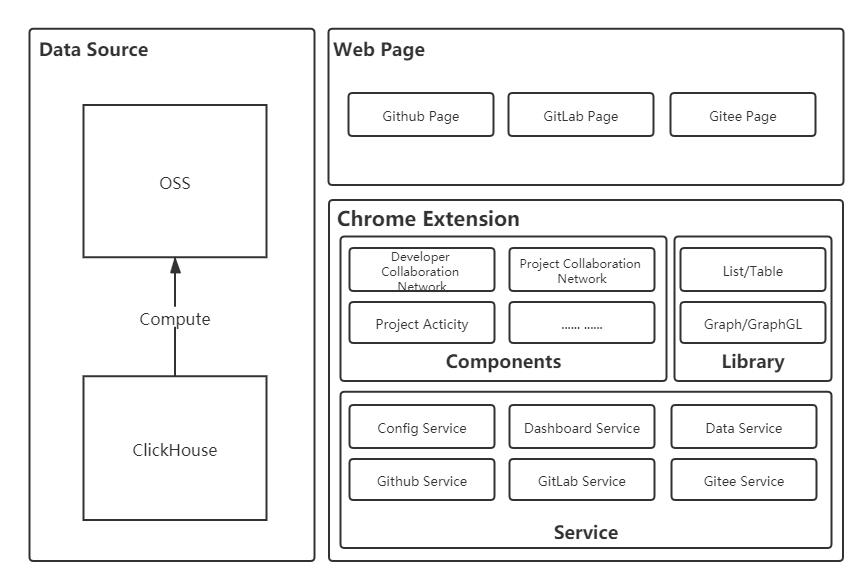
\includegraphics[width=150mm]{./figures/image5-1.png}
    \caption{技术架构图\\Technical architecture diagram}
\end{figure}
% //TODO: 确认是否可行?
\par 面向开放社区的迷你看板的搭建过程本质上是一个浏览器插件的开发,从后端到前端,分为数据源、插件主体、前端页面三个部分。
\par 在数据源部分,后端由Hypertrons收集的开放平台全域数据存储在ClickHouse数据库中,按照上文所述的定义与计算方法,计算得到具体的字段数值,作为静态对象存储到OSS(Object Storage Service,阿里云对象存储)服务中,供前端直接调用。
\par 在插件主体部分,使用Typescript类定义各可视化图表组件,作为可以调用的模板,提供接口以嵌入真实的数据。同时,在该部分构建了配置服务、仪表盘服务,并联通后端的数据服务和3个开放平台(Github、GitLab和Gitee)的服务接口。其中,配置服务负责维护一个存储用户配置信息的json文件,每一次向后端发起请求、渲染图表之前,都去读取;仪表盘服务则负责取得数据、嵌入可视化组件模板,生成图表以插入到前端页面。
\par 在前端页面部分,则根据Github、GitLab、Gitee三个开放平台的UI风格,选择了与原生样式相近的组件库FrontUI,在原网页布局的基础上,将仪表盘服务生成的图表插入到页面的特定位置,如边栏、文本间等。

\par 在这个基础上,考虑到开发便利性与项目的国际化程度,在功能实现、架构搭建的基础上,还使用了chrome的i18n架构以增添插件对不同语言的支持,使用了静态代码分析工具ESLint、代码格式化工具Prettier和同为开源项目的工具Husky来使代码规范化。这些工作是为了保障本项目作为开源项目的开放性。



\subsection{高可配能力的实现}
\par 项目所有的配置都从代码仓库中的配置文件 .github/hypertrons.json 中读取,即:
插件所提供的功能由配置文件决定,配置文件配置在项目中,基于 Git 进行管理和迭代,公开透明。
同一项目下的所有安装该插件的用户,Perceptor 提供的是相同的能力。
同一用户,在不同项目页面下,看到的是不同的看板。


\subsection{数字化看板模块的实现}
% 各个功能对应的技术手段
\par 项目基于Echarts提供数据可视化图表渲染能力。Echarts是一个使用JavaScript实现的开源可视化库,提供直观、交互丰富、可高度个性化定制的数据可视化图表。通过对Echarts进行封装,并基于Hypertrons后端获取数字化看板的配置信息以及各个平台的开放数据,就可以根据每个社区/组织的自身业务场景,实现高度可配的数字化看板。基于此,能够实现支持每一位用户基于自身权限地配置浏览器页面的数字化看板。
\par 以GitHub项目数字化看板展示为例,可从hypertrons后端获取得到数字化看板的配置信息,以及项目的Repository、Issue、Pull request和从其他平台采集得到的开放数据,然后根据用户自定义的配置信息生成相应的可视化组件,再经由浏览器插件,以HTML的格式注入到用户浏览的当前页面,完成整个呈现。



\subsection{跨平台交互模块的实现}
\par 在浏览器页面中输入的交互式命令行会由浏览器插件传递到hypertrons 后端,由hypertrons 后端运行、完成指定操作后后,再通过浏览器插件,反馈结果给来自不同平台、使用不同语言的用户,从而提供跨平台交互的能力。

\subsection{跨平台实时消息通知与配置管理模块的实现}
\par 跨平台实时消息通知与配置管理模块是基于浏览器插件的特性,在Chromium提供的用于浏览器插件开发的官方接口上进行实现。其本质是前后端之间信息的简单传递。

\subsection{身份认证与权限管理模块的实现}
\par 用户能够在开源平台的设置项中管理自己的Token,而当用户为迷你看板插件配置了个人账户的Token,即迷你看板插件获得了该用户账号的部分权限。获得用户Token之后,插件将读取的用户名和头像自动显示,并且该Token会在后续发生的一系列请求访问中自动使用。

\subsection{功能测试}
% Jest(?有什么测试案例或指标吗)
\par 项目使用Jest,一个简洁的测试框架,它能够很好地与Typescript以及React框架共用。Jest在大部分基于JavaScript的项目上可以实现开箱即用、无需配置,且具有优秀的 api,易于书写与维护。
% //TODO: 'Error: no test specified'


% //TODO: 最后要不要放效果图?
% \subsection{实现结果}
% 项目、个人Github主页最终效果(贴图)


             %正文第五章
\section{总结与展望}
% 项目本身的意义、对开源社区做出的贡献
\subsection{总结}
% \par 本文围绕着开放平台的数据可视化问题,对迷你看板——一个浏览器插件落地所经历的的分析、设计与实现过程进行了详细的阐述。
\par 本课题针对开放组织,结合机器人流程自动化,实现一个基于浏览器插件的迷你看板,采用了浏览器插件的形式,通过在特定网址的网页中插入可视化组件并提供交互手段,协助开源社区中不同项目、不同视角的决策与运营,进一步完善了开源社区中的数字化治理框架,可以帮助开放组织或开源社区更高效的运作和管理。
\par 论文首先阐述了项目的研究背景与研究动机,主要介绍了开源社区与开放组织的的运作模式与发展方向,随之提出了本文主要面向的问题与需求。接着,提出明确的方法定义,去对开放平台的数据进行探索分析,挖掘其隐藏并有价值的数据信息,并形成具体的的可视化分析的方向。明确了研究方向与目的以后,再从产品与业务的角度出发,剖析需求、流程、业务逻辑,完成迷你看板的总体定位与细节功能设计。最后,针对每一个开发环节与功能模块,调研技术方法、确定技术方法,并逐个实现。

\subsection{展望}
\par 开放式组织中包含了人员招聘、项目管理、人力绩效、工资分红、退出机制、宣传营销等各个环节,下一步可考虑在本文实现的迷你看板的基础上,添加人员的进入与退出机制、工资分红机制等,从而完善开放组织或开源社区的治理框架,帮助开放组织完成宣传、活动、用户、开发、管理、布道等各个方面进行数字化管理和常态化。

\par 经由这个项目,在开源社区中可视化深层信息、辅助决策的目的已经基本能够达到。这个迷你看板以浏览器插件的形式实现,在完善开源社区机制、推动生产力关系变革的进程中迈进了有意义的一步,在这个项目的基础上,已然可以展望开源供应链的迭代、区块链等新技术的加入,但这些也绝不会是终点。开源的进程在当前的基础上将不断被推动,并将最终演化出新的组织关系和技术产物,相互促进,往复循环。
%  Section A
\section{章节结构测试}这节用来展示文章的5层结构。事实上,一般来说文章层次在3-4层为宜。在之后的section中,我们会只使用至多3层结构(即,节-小节-子节)来进行各种演示。
 
\subsection{小节标题}这一小节我们介绍这些内容。

\subsubsection{子节标题}这一子节我们介绍这些内容。

\paragraph{段标题}这一段我们介绍这些内容。 

\subparagraph{小段标题}这一小段我们介绍这些内容。

%   Section B
\section{定理等环境测试}这节用来展示定理,引理等常用论文环境。
 
\subsection{编号环境与不编号环境}

\subsubsection{编号环境}

\begin{theorem}\label{thm2_1}

    设$A,B$是两个实数, 则$2AB\leq 2 A^2+B^2$.
    
\end{theorem}

\begin{proof}
    这里是证明。
\end{proof}

\begin{lemma}[Nakayama引理]\label{lem2_2}
    这是一条引理测试。。。
\end{lemma}

\begin{problem}[连续统假设]是否存在$\mathbb{R}$的子集S使得$card(\mathbb{N})<card(S)<card(\mathbb{R})$?
\end{problem}
\begin{solution}
    不存在。
\end{solution}

\subsubsection{无编号环境}

\begin{theorem*}

    设$A,B$是两个实数, 则$2AB\leq 2 A^2+B^2$.
    
\end{theorem*}

\begin{proof}
    这里是证明。
\end{proof}

\begin{lemma*}[Nakayama引理]
    这是一条引理测试。。。
\end{lemma*}

\begin{problem*}[连续统假设]是否存在$\mathbb{R}$的子集S使得$card(\mathbb{N})<card(S)<card(\mathbb{R})$?
\end{problem*}
\begin{solution}
    不存在。
\end{solution}

% Section C
\section{公式测试}这节用来展示公式,交换图等。
 
\subsection{行内公式}
典范的同态$\lim_{\leftarrow F} W_r(S)\rightarrow \lim_{\leftarrow F} W_r(S/\pi S )$是同构。

\subsection{整行公式}
$$\mathbb{A}_{inf}=W(S^\flat)\cong \lim_{\leftarrow F} W_r(S)$$

\subsection{多行公式}
\begin{sloppypar}
多行公式的情况非常多,对齐与换行的要求也各不相同。所以选择合适的环境非常重要。这份文档里无法涵盖所有情况,所以提供一个教程用以参考:\url{http://blog.csdn.net/yanxiangtianji/article/details/54767265}
\end{sloppypar}



\subsubsection{align环境}
\begin{align*}
    \operatorname{E} (Z_{n+1} - Z_n | X_1,..., X_n)
    &= \operatorname{E} (S_{n+1}^2 - (n+1) \sigma^2 - S_n^2 + n \sigma^2 | X_1,..., X_n) \\
    &= \operatorname{E} (S_{n+1}^2 - S_n^2 - (n+1) \sigma^2 + n \sigma^2 | X_1,..., X_n) \\
    &= \operatorname{E} (X_{n+1}(X_{n+1} + 2\sum_{i=1}^n X_i) - \sigma^2 | X_1,..., X_n) \\
    &= \operatorname{E} (X_{n+1}X_{n+1})
       + 2\operatorname{E} (X_{n+1}) \sum_{i=1}^n X_i - \sigma^2 \\
    &= \sigma^2  - \sigma^2 =0.
\end{align*}

\subsubsection{split环境(内嵌)}
\begin{equation*}
    \begin{split}
    (a + b)^4
      &= (a + b)^2 (a + b)^2      \\
      &= (a^2 + 2ab + b^2)
         (a^2 + 2ab + b^2)        \\
      &= a^4 + 4a^3b + 6a^2b^2 + 4ab^3 + b^4
    \end{split}
\end{equation*}

\subsubsection{带大括号的多行公式}
\paragraph{cases}
$$
    f=
    \begin{cases}
      x + y = z,  \\
      1 + 2 = 3.  \\
    \end{cases}
$$

\paragraph{array}
$$ F^{HLLC}=\left\{
\begin{array}{rcl}
F_L       &      & {0      <      S_L}\\
F^*_L     &      & {S_L \leq 0 < S_M}\\
F^*_R     &      & {S_M \leq 0 < S_R}\\
F_R       &      & {S_R \leq 0}
\end{array} \right. $$
    
\paragraph{aligned}
\begin{equation}
    \left\{
     \begin{aligned}
     \overset{.}x(t) &=A_{ci}x(t)+B_{1ci}w(t)+B_{2ci}u(t)  \\
     z(t) &=C_{ci}x(t)+D_{ci}u(t) \\
     \end{aligned}
     \right.
\end{equation}

\subsection{交换图}
\begin{sloppypar}
强烈推荐tikzcd-editor:\url{https://github.com/yishn/tikzcd-editor}
\end{sloppypar}

\begin{center}
\begin{tikzcd}
    T
    \arrow[drr, bend left, "x"]
    \arrow[ddr, bend right, "y"]
    \arrow[dr, dotted, "{(x,y)}" description] & & \\
    & X \times_Z Y \arrow[r, "p"] \arrow[d, "q"]
    & X \arrow[d, "f"] \\
    & Y \arrow[r, "g"]
    & Z
\end{tikzcd}
\end{center}

\begin{center}
    \begin{tikzcd}[row sep=scriptsize, column sep=scriptsize]
        & f^* E_V \arrow[dl] \arrow[rr] \arrow[dd] & & E_V \arrow[dl] \arrow[dd] \\
        f^* E \arrow[rr, crossing over] \arrow[dd] & & E \\
        & U \arrow[dl] \arrow[rr] & & V \arrow[dl] \\
        M \arrow[rr] & & N \arrow[from=uu, crossing over]\\
        \end{tikzcd}
\end{center}

\begin{center}
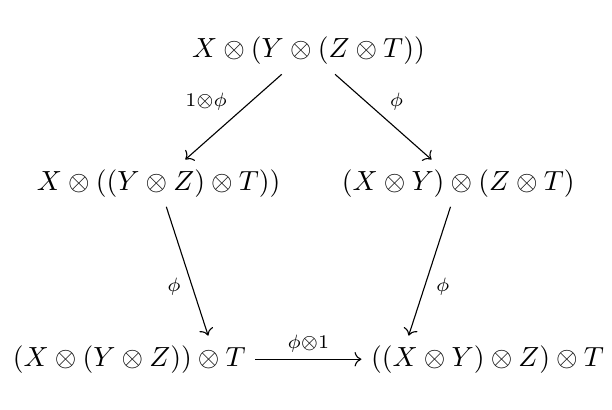
\begin{tikzpicture}[commutative diagrams/every diagram]
    \node (P0) at (90:2.3cm) {$X\otimes (Y\otimes (Z\otimes T))$};
    \node (P1) at (90+72:2cm) {$X\otimes ((Y\otimes Z)\otimes T))$} ;
    \node (P2) at (90+2*72:2cm) {\makebox[5ex][r]{$(X\otimes (Y\otimes Z))\otimes T$}};
    \node (P3) at (90+3*72:2cm) {\makebox[5ex][l]{$((X\otimes Y)\otimes Z)\otimes T$}};
    \node (P4) at (90+4*72:2cm) {$(X\otimes Y)\otimes (Z\otimes T)$};
    \path[commutative diagrams/.cd, every arrow, every label]
    (P0) edge node[swap] {$1\otimes\phi$} (P1)
    (P1) edge node[swap] {$\phi$} (P2)
    (P2) edge node {$\phi\otimes 1$} (P3)
    (P4) edge node {$\phi$} (P3)
    (P0) edge node {$\phi$} (P4);
\end{tikzpicture}
\end{center}


% Section D
\subsection{表格}
\par 本来LaTeX里表格的变化是非常多的,但鉴于学校要求用三线式,问题反而简单了。以下是一个例子:
\begin{table}[htbp]\center
    \caption{示例表格\\Example Table}
    \begin{tabular}{lcccccl}
     \toprule
     。。 & 。。 & 。。 & 。。 & 。。& 。。 & 。。\\
     \midrule
    。。 & 。。 & 。。 & 。。 & 。。& 。。 & 。。\\
    。。 & 。。 & 。。 & 。。 & 。。& 。。 & 。。\\
    。。 & 。。 & 。。 & 。。 & 。。& 。。 & 。。\\
    。。 & 。。 & 。。 & 。。 & 。。& 。。 & 。。\\
    。。 & 。。 & 。。 & 。。 & 。。& 。。 & 。。\\
     \bottomrule
    \end{tabular}
   \end{table}
如果你有使用更复杂的表格的需求,请自行查资料完成。

\subsection{插图}
由于这份模板不考虑多栏排版,所以格式要求中所述的半栏图大小要求我们不作演示。以下是一个通栏图的演示:
\begin{figure}[H]
    \centering
    \includegraphics[width=100mm]{example-image}
    \caption{图片测试(最小宽度)\\Image test (Minimal width)}
  \end{figure}

\begin{figure}[H]
    \centering
    \includegraphics[width=130mm]{example-image}
    %\includegraphics[width=130mm]{./figures/你自己的图像文件}
    \caption{图片测试(最大宽度)\\Image test (Maximal width)}
\end{figure}
\par 注意:这里为了减少图片上下的空白,使用了float宏包。
© 2021 GitHub, Inc.


% Section E
\section{注释与引用}这节用来展示注释与引用。

\subsection{注释——脚注与尾注}
\subsubsection{脚注}
\par 这里是脚注测试\footnote{1111111111}这里是脚注测试这里是脚注测试这里是脚注测试\footnote{2222222222}这里是脚注测试这里是脚注测试这里是脚注测试这里是脚注测试这里是脚注测试这里是脚注测试这里是脚注测试这里是脚注测试这里是脚注测试这里是脚注测试这里是脚注测试这里是脚注测试这里是脚注测试这里是脚注测试这里是脚注测试\footnote{3333333333}这里是脚注测试这里是脚注测试这里是脚注测试这里是脚注测试这里是脚注测试这里是脚注测试这里是脚注测试这里是脚注测试这里是脚注测试这里是脚注测试这里是脚注测试这里是脚注测试

\textcolor{red}{\textbf{\uline{注意!正如这份演示中所出现的情况,若该页(也就是本文档中的前一页)剩余空间不大,不足以显示足够多的文档与脚注,那么该段文字就会被移至下一页而留下空白。目前我们尚未找到解决的方法,所以如果遇到了这个问题,请修改排版,以留下足够大的空间。}}}

\subsubsection{尾注}
\par 这里是尾注测试\endnote{伴随着互联网的发展以及新的网络应用的出现,互联网用户由单纯的“读”网页,向“读、写”网页,共同建设互联网发展,由此网上产生了大量带有用户主观感情的数据,从这些带...}这里是尾注测试这里是尾注测试这里是尾注测试这里是尾注测试\endnote{尾注测试2}这里是尾注测试这里是尾注测试这里是尾注测试这里是尾注测试这里是尾注测试这里是尾注测试这里是尾注测试这里是尾注测试这里是尾注测试这里是尾注测试这里是尾注测试这里是尾注测试这里是尾注测试这里是尾注测试这里是尾注测试\endnote{尾注测试3}这里是尾注测试这里是尾注测试这里是尾注测试这里是尾注测试这里是尾注测试这里是尾注测试这里是尾注测试这里是尾注测试这里是尾注测试

\par \textcolor{red}{\textbf{\uline{注意!endnotes宏包并不支持hyperref,也就是无法通过点击文中尾注标号以跳转到尾注。当然,这在打印出来的文档中并不会造成任何影响。}}}
\par \textcolor{blue}{\textbf{\uline{提示:尾注出现在全文最后。为了区分脚注与尾注的编号,我们在尾注编号前加上了“尾注”二字。}}}

\subsection{交叉引用}
\par 本模板使用cleveref宏包来进行交叉引用。使用的指令为$\backslash$cref$\{$label$\}$。例子如下:
\par 由\cref{thm2_1}我们可以知道XXXXXXXX。
\par 由\cref{lem2_2}我们可以知道XXXXXXXX。
\par 请注意,label是需要手工设置的,一般将label放在你需要引用的环境内即可(具体可见SectionB.tex)。

\subsection{文献引用的演示}
\par 本模板使用biblatex进行文献管理,这是一套相对较新的系统。另外,使用了hushidong制作的符合gb7714-2015标准的biblatex样式。在此对他的工作表示感谢,要完成这样的样式非常不容易。本模板中gb7714-2015.bbx与gb7714-2015.cbx即为他的作品,在这里打包发布以便使用。
\par 默认的bib文件位于~/reference/thesis-ref.bib,内容是由Wang Tianshu制作,在此仅作演示之用。关于bib文件的编写与管理请自行查找相关教程。
\par 下方的演示已经给出了正文中引用文献的基本方法,这与传统的cite命令是类似的。如有更多需求,请至\url{https://github.com/hushidong/biblatex-gb7714-2015}查找相关资料。
\par 文献\parencite{Yang_Hy200215}中提到xxxxxxx。
\par 文献\parencite{Joa1999}中提到yyyyyyy。
\par 文献\parencite{Altman1997}中提到zzzzzzz。
\par \textcolor{blue}{\textbf{\uline{本模板使用parencite而不是cite命令,因为这样能与脚注所产生编号进行区分。当然,如果你没有脚注或尾注,那么cite命令也是推荐使用的。}}}

% SectionFConclusion
% \theendnotes %尾注(若没有尾注请将本行删除)
\ClearPageStyle

%生成参考文献
\phantomsection
\addcontentsline{toc}{section}{参考文献}
\printbibliography[title={\centerline{\bfseries\sffamily \zihao {-3}参考文献}}]
\ClearPageStyle

%生成附录
\phantomsection
\addtocontents{toc}{\setcounter{tocdepth}{1}}
\addcontentsline{toc}{section}{附录}
\setcounter{subsection}{0}
\ctexset { subsection = { name={,},number={\arabic{subsection}},format={\rmfamily \zihao {5}} } }
\ctexset { subparagraph = { name={(,)},number={\arabic{subparagraph}},format={\rmfamily \zihao {5}},indent=2em } }
\section*{\centerline{\bfseries \sffamily \zihao{-3} 附录}}

\subsection{部分代码}
\begin{itemize}
\item 定义PercepterBase类做一些简单的工作如logger、场景判断。
\end{itemize}
\begin{lstlisting}
export default abstract class PerceptorBase {
    public logger: any;

    constructor() {
    this.logger = {
        info: (message?: any, ...optionalParams: any[]): 
        void => {
        if (process.env.NODE_ENV !== 'production') {
            console.log('ℹ️ Perceptor : ',
             message, ...optionalParams);
        }
        },
        error: (message?: any, ...optionalParams: any[]): 
        void => {
        console.error('❌ Error Message From Perceptor :',
         message, ...optionalParams);
        // TODO: pass error message to ErrorMessageBar component
        render(<ErrorMessageBar />, 
        document.getElementById('perceptor'))
        }
    };
    }

    public abstract run(): Promise<void>;
}
\end{lstlisting}

\begin{itemize}
\item 定义Perceptor类继承PerceptorBase,来检查settings、创建div、取配置文件、渲染每一个组件。
\end{itemize}
\begin{lstlisting}
export class Perceptor extends PerceptorBase {
    public static Features: Map<string, any> = new Map();
    public settings: any;

    public async run(): Promise<void> {
    // wait until <body> element is ready
    await elementReady('body', { waitForChildren: false });
    this.logger.info('body element is ready.');

    this.logger.info('creating perceptor div ...');
    const perceptorDiv = document.createElement('div');
    perceptorDiv.id = 'perceptor';
    $('#js-repo-pjax-container').prepend(perceptorDiv);

    await this.checkSettings();

    // run every features
    Perceptor.Features.forEach(async (Feature, name) => {
        const featureId = name.replace(name[0],
        name[0].toLowerCase());
        this.logger.info('trying to load ', featureId)
        if (this.settings.toJson()[featureId] === false) {
        this.logger.info(featureId, 'is disabled');
        return;
        }
        if (Feature.prototype.include
        .every((c: () => any) => !c())) {
        this.logger.info(featureId,
         'does NOT run on this page')
        return;
        }
        try {
        this.logger.info('running ', featureId)
        const feature = new Feature();
        await feature.run();
        } catch (error: unknown) {
        this.logger.error(featureId, error)
        }
    }, this)

    private async checkSettings(): Promise<void> {
        this.logger.info('loading settings ...');
        if (isRepo()) {
            this.logger.info('Detected that this is a repo page,
             trying to load configuration file from the repo ...');

            const owner = utils.getRepositoryInfo(window.location)!
            .owner;
            const repo = utils.getRepositoryInfo(window.location)!
            .name;
            const configFromGithub = await getConfigFromGithub(owner, repo);
            this.logger.info('The configurations are: ', configFromGithub);
            this.settings = await mergeSettings(configFromGithub);
        } else {
            this.settings = await loadSettings();
        }
    }
}
\end{lstlisting}
\begin{itemize}
    \item 渲染组件,以开发者协作网络为例:
\end{itemize}
\begin{lstlisting}
public async run(): Promise<void> {
    const pinnedReposDiv = $('.js-pinned-items-reorder-container')
    .parent();
    const DeveloperNetworkDiv = document.createElement('div');
    DeveloperNetworkDiv.id = 'developer-network';
    DeveloperNetworkDiv.style.width = "100%";
    this._currentDeveloper = $('.p-nickname.vcard-username.d-block')
    .text().trim();
    const settings=await loadSettings();
    try {
    const forceGraphDataRaw = await getGraphData(`/actor/${this._currentDeveloper}.json`);
    await this.generateForceGraphData(forceGraphDataRaw);

    const circularGraphDataRaw = await getGraphData(
        `/actor/${this._currentDeveloper}_top.json`);
    await this.generateCircularGraphData(circularGraphDataRaw);

    const developerColumns = [
        {
        key: 'column1',
        name: getMessageI18n('global_developer'),
        fieldName: 'name',
        minWidth: 100,
        maxWidth: 200,
        isResizable: true,
        onRender: (item: any) => (
            <Link href={'https://github.com/' + item.name} >
            {item.name}
            </Link>
        ),
        },
        { key: 'column2', name: getMessageI18n('global_correlation'), fieldName: 'correlation', minWidth: 100, maxWidth: 200, isResizable: true },
        { key: 'column3', name: getMessageI18n('global_activity'), fieldName: 'activity', minWidth: 100, maxWidth: 200, isResizable: true },
    ];
    const repoColumns = [
        {
        key: 'column1',
        name: getMessageI18n('global_repo'),
        fieldName: 'name',
        minWidth: 100,
        maxWidth: 200,
        isResizable: true,
        onRender: (item: any) => (
            <Link href={'https://github.com/' + item.name} >
            {item.name}
            </Link>
        ),
        },
        { key: 'column2', name:
         getMessageI18n('global_contribution'), fieldName: 'value', minWidth: 100, maxWidth: 200, isResizable: true },
    ];
    render(
        <div>
        < GraphWithList
            layout='force'
            graphType={settings.graphType}
            title={getMessageI18n('component_developerCollabrationNetwork_title')}
            graphData={this._forceGraphData}
            graphDataGraphin={this._forceGraphDataGraphin}
            columns={developerColumns}
            listData={this._developerListData}
        />
        < GraphWithList
            layout='circular'
            graphType={settings.graphType}
            title={getMessageI18n('component_mostParticipatedProjects_title')}
            graphData={this._circularGraphData}
            graphDataGraphin={this._circularGraphDataGraphin}
            columns={repoColumns}
            listData={this._repoListData}
        />
        </div>,
        DeveloperNetworkDiv,
    );
    pinnedReposDiv.before(DeveloperNetworkDiv);
    } catch (error) {
    this.logger.error('DeveloperNetwork', error);
    return;
    }
}
\end{lstlisting}


\ClearPageStyle

\makeacknowledgement %生成感谢

\end{document} 
